\documentclass[12pt,a4paper]{report}
\usepackage{amsmath,amsthm,amssymb,graphicx,hyperref}
\usepackage[left=1.2in,right=1in,top=1in,bottom=1in]{geometry}
\usepackage[romanian]{babel}
\usepackage{indentfirst}
\usepackage{algorithm}
\usepackage{algpseudocode}
\usepackage{listings}
\usepackage{float}
\usepackage[T1]{fontenc}
\usepackage{microtype}
\usepackage{tikz}
\usetikzlibrary{positioning, arrows.meta, shapes.geometric, fit, backgrounds}
%\usepackage{...insert other packages here...}
\newtheorem{thm}{Teorema}[section]
\newtheorem{lem}[thm]{Lema}
\newtheorem{cor}[thm]{Corolarul}
\newtheorem{prop}[thm]{Propozi\c tia}
\theoremstyle{definition}
\newtheorem{defn}{Defini\c tia}[section]
\theoremstyle{remark}
\newtheorem{rem}{Remarca}[section]
\newtheorem{exmp}{Exemplul}[section]

\def\contentsname{Cuprins}
\def\listfigurename{Lista figurilor}
\def\listtablename{Lista tabelelor}
\def\figurename{Figura}
\def\tablename{Tabelul}
\def\partname{Partea}
\def\chaptername{Capitolul}
\def\refname{Referințe}
\def\bibname{Bibliografie} 
\def\appendixname{Anexa}

\begin{document}
\thispagestyle{empty}
\begin{center}
\begin{figure}[h!]
\vspace{-20pt}
\begin{center}
\includegraphics[width=100pt]{FI.png}
\end{center}
\end{figure}


{\large{\bf UNIVERSITATEA DE VEST DIN TIMIȘOARA

FACULTATEA DE INFORMATICĂ

PROGRAMUL DE STUDII DE MASTER:  Bioinformatică }}

\vspace{120pt}
{\huge {\bf LUCRARE DE DIZERTAȚIE}}

\vspace{150pt}
\end{center}

{\large\noindent{\bf COORDONATOR:\hfill ABSOLVENT:}

\noindent Prof. Dr. Zaharie Daniela \hfill Gâță Răzvan-Andrei}

\vfill
\begin{center}
{\bf TIMI\c SOARA

2026}
\end{center}
\newpage

% ============================================================
% COPERTA A 2-A — cu titlul lucrarii
% ============================================================
\thispagestyle{empty}
\begin{center}
{\large{\bf UNIVERSITATEA DE VEST DIN TIMIȘOARA

FACULTATEA DE INFORMATICĂ


PROGRAMUL DE STUDII DE MASTER: Bioinformatică }}

\vspace{80pt}
{\huge {\bf LUCRARE DE DIZERTAȚIE}}

\vspace{30pt}
{\LARGE {\bf Clasificarea Semnalelor EEG utilizând\\[6pt]
Rețele Neuronale de tip Graf}}

\vspace{150pt}
\end{center}

{\large\noindent{\bf COORDONATOR:\hfill ABSOLVENT:}

\noindent Prof. Dr. Zaharie Daniela \hfill Gâță Răzvan-Andrei}

\vfill
\begin{center}
{\bf TIMIȘOARA

2026}
\end{center}
\newpage
\normalsize{}

\section*{Abstract - Română}

Electroencefalografia (EEG) reprezintă una dintre cele mai utilizate metode pentru monitorizarea activității electrice a creierului, datorită caracterului său non-invaziv, portabilității și rezoluției temporale ridicate. Cu toate acestea, analiza semnalelor EEG rămâne o provocare majoră, deoarece acestea sunt serii de timp multicanal complexe, afectate de zgomot, artefacte și variabilitate ridicată între subiecți. În plus, structura lor non-euclidiană limitează aplicabilitatea metodelor convenționale de învățare profundă, precum rețelele neuronale convoluționale.

Prezenta lucrare investighează utilizarea rețelelor neuronale de tip graf (Graph Neural Networks -- GNN) pentru analiza și clasificarea datelor EEG, cu accent pe captarea relațiilor complexe dintre diferitele regiuni cerebrale. În cadrul abordării propuse, semnalele EEG sunt reprezentate sub forma unor grafuri, în care electrozii sunt modelați ca noduri, iar relațiile dintre aceștia sunt descrise prin muchii. Această reprezentare permite păstrarea topologiei datelor și integrarea informațiilor spațiale și funcționale într-un mod mai adecvat decât metodele bazate pe structuri regulate.

Lucrarea include o analiză teoretică a particularităților datelor EEG, a etapelor de pre-procesare necesare și a principalelor arhitecturi GNN relevante pentru acest domeniu, în special Graph Convolutional Networks (GCN) și Graph Attention Networks (GAT). De asemenea, este propus și implementat un pipeline complet pentru procesarea datelor EEG, construirea reprezentării de tip graf, antrenarea și evaluarea modelelor, utilizând limbajul Python și biblioteca PyTorch Geometric. În plus, a fost dezvoltată o interfață grafică dedicată vizualizării și interpretării rezultatelor obținute.

Motivația principală a lucrării este dată de potențialul utilizării GNN în aplicații biomedicale, în special în contextul identificării unor tipare asociate afecțiunilor neurologice și neurodegenerative, precum boala Alzheimer. Prin această lucrare se urmărește evidențierea avantajelor oferite de modelele bazate pe graf în analiza semnalelor EEG și susținerea utilizării acestora ca alternativă promițătoare la abordările tradiționale.

\newpage
\normalsize{}

\section*{Abstract - English}

Electroencephalography (EEG) is one of the most widely used techniques for monitoring brain activity, due to its non-invasive nature, portability, and high temporal resolution. However, the analysis of EEG signals remains a challenging task, as these signals are complex multichannel time series affected by noise, artifacts, and high inter-subject variability. Moreover, their non-Euclidean structure limits the applicability of conventional deep learning approaches, such as convolutional neural networks.

This thesis investigates the use of Graph Neural Networks (GNN) for the analysis and classification of EEG data, with a focus on capturing the complex relationships between different brain regions. In the proposed approach, EEG signals are represented as graphs, where electrodes are modeled as nodes and the relationships between them are represented as edges. This representation enables the preservation of the intrinsic structure of the data and allows for a more effective integration of spatial and functional information.

The work includes a theoretical analysis of EEG data characteristics, preprocessing techniques, and the main GNN architectures relevant to this domain, particularly Graph Convolutional Networks (GCN) and Graph Attention Networks (GAT). Furthermore, a complete pipeline is proposed and implemented for EEG data processing, graph construction, model training, and evaluation, using Python and the PyTorch Geometric library. In addition, a graphical user interface is developed to facilitate the visualization and interpretation of the obtained results.

The main motivation of this study lies in the potential of GNN-based approaches in biomedical applications, especially for identifying patterns associated with neurological and neurodegenerative disorders, such as Alzheimer's disease. This thesis aims to highlight the advantages of graph-based models in EEG signal analysis and to support their use as a promising alternative to traditional methods.

\newpage

% ============================================================
% SECTIUNEA DE NOTATII SI ABREVIERI
% ============================================================
\section*{Notații și abrevieri}
\addcontentsline{toc}{chapter}{Notații și abrevieri}

În cuprinsul prezentei lucrări sunt utilizate în mod consistent următoarele notații matematice și abrevieri:

\vspace{8pt}
\noindent\textbf{Notații matematice generale}
\begin{itemize}
    \item $i$ -- unitatea imaginară, cu proprietatea $i^2 = -1$
    \item $\mathbb{R}^{m \times n}$ -- spațiul matricelor reale de dimensiune $m \times n$
    \item $|\cdot|$ -- modulul unui număr complex sau valoarea absolută a unui număr real
    \item $\arg(\cdot)$ -- argumentul (faza) unui număr complex
    \item $\lfloor \cdot \rfloor$ -- partea întreagă inferioară (floor)
    \item $\|\cdot\|$ -- operația de concatenare a vectorilor (în context GNN)
\end{itemize}

\vspace{8pt}
\noindent\textbf{Notații specifice semnalelor EEG și conectivității funcționale}
\begin{itemize}
    \item $x(t)$ -- semnalul EEG real, în funcție de timp $t$
    \item $z(t)$ -- semnalul analitic complex asociat lui $x(t)$
    \item $\mathcal{H}[\cdot]$ -- transformata Hilbert a unui semnal real
    \item $\phi(t)$ -- faza instantanee a semnalului $x(t)$
    \item $\phi_i(t),\, \phi_j(t)$ -- fazele instantanee ale canalelor EEG $i$, respectiv $j$
    \item $T$ -- numărul de eșantioane temporale ale unei epoci EEG
    \item $PLV_{ij} \in [0, 1]$ -- Phase Locking Value dintre canalele $i$ și $j$
    \item $f_l,\, f_h$ -- frecvența inferioară, respectiv superioară a unui filtru trece-bandă (Hz)
    \item $f_s$ -- rata de eșantionare a semnalului EEG (Hz)
    \item $\Delta t$ -- durata unei epoci EEG (secunde)
    \item $\mathbf{X} \in \mathbb{R}^{N_e \times N_c \times N_t}$ -- tensorul epocilor EEG, cu $N_e$ epoci, $N_c$ canale și $N_t$ eșantioane temporale
\end{itemize}

\vspace{8pt}
\noindent\textbf{Notații specifice rețelelor neuronale de tip graf}
\begin{itemize}
    \item $G = (V, E)$ -- graful EEG, unde $V$ este mulțimea nodurilor (electrozi), iar $E$ este mulțimea muchiilor (relații funcționale)
    \item $N = |V|$ -- numărul de noduri ale grafului ($N = 19$ în implementarea prezentă)
    \item $A \in \mathbb{R}^{N \times N}$ -- matricea de adiacență a grafului
    \item $\tilde{A} = A + I_N$ -- matricea de adiacență cu auto-conexiuni adăugate, unde $I_N$ este matricea identitate de dimensiune $N$
    \item $\tilde{D}$ -- matricea diagonală de grade asociată lui $\tilde{A}$, cu $\tilde{D}_{ii} = \sum_j \tilde{A}_{ij}$
    \item $\mathbf{h}_v^{(l)} \in \mathbb{R}^{d_l}$ -- vectorul de caracteristici al nodului $v$ la stratul $l$, de dimensiune $d_l$
    \item $\mathcal{N}(v)$ -- mulțimea vecinilor nodului $v$ în graf
    \item $W^{(l)} \in \mathbb{R}^{d_l \times d_{l+1}}$ -- matricea de ponderi antrenabilă a stratului $l$
    \item $\sigma(\cdot)$ -- funcție de activare neliniară (e.g., ReLU sau ELU)
    \item $\alpha_{ij}$ -- coeficientul de atenție normalizat al muchiei $(i, j)$ în GAT
    \item $e_{ij}$ -- scorul de atenție nenormalizat al muchiei $(i, j)$ în GAT
    \item $\mathbf{a} \in \mathbb{R}^{2d'}$ -- vectorul de atenție antrenabil în GAT
    \item $K$ -- numărul de capuri de atenție (attention heads) în mecanismul multi-head al GAT
\end{itemize}

\vspace{8pt}
\noindent\textbf{Abrevieri}
\begin{itemize}
    \item \textbf{EEG} -- Electroencefalografie / Electroencephalography
    \item \textbf{GNN} -- Rețea Neuronală de tip Graf / Graph Neural Network
    \item \textbf{GCN} -- Rețea Convoluțională pe Graf / Graph Convolutional Network
    \item \textbf{GAT} -- Rețea de Atenție pe Graf / Graph Attention Network
    \item \textbf{PLV} -- Phase Locking Value (Valoarea de Blocare a Fazei)
    \item \textbf{ICA} -- Analiza Componentelor Independente / Independent Component Analysis
    \item \textbf{FIR} -- Finite Impulse Response (Răspuns Finit la Impuls)
    \item \textbf{PSD} -- Power Spectral Density (Densitatea Spectrală de Putere)
    \item \textbf{PyG} -- PyTorch Geometric
    \item \textbf{MNE} -- biblioteca MNE-Python pentru procesarea semnalelor neurofiziologice
    \item \textbf{BIDS} -- Brain Imaging Data Structure
    \item \textbf{BCI} -- Brain-Computer Interface (Interfață Creier-Calculator)
    \item \textbf{CNN} -- Rețea Neuronală Convoluțională / Convolutional Neural Network
    \item \textbf{ReLU} -- Rectified Linear Unit (funcție de activare)
    \item \textbf{ELU} -- Exponential Linear Unit (funcție de activare)
\end{itemize}

\tableofcontents
\newpage
\chapter{Introducere}

Prezentul capitol introduce contextul general al lucrării, descriind motivația utilizării rețelelor neuronale de tip graf pentru analiza semnalelor EEG, obiectivele urmărite, contribuțiile principale și abordarea generală adoptată.

\section{Motivație și context general}

În domeniul neuroștiințelor, înțelegerea activității neuronale și a modului în care aceasta corelează cu comportamentul și funcțiile cognitive este esențială, atât pentru diagnosticarea și tratarea afecțiunilor neurologice, precum Alzheimer sau epilepsie, cât și pentru dezvoltarea aplicațiilor de tip BCI (Brain-Computer Interfaces). În acest context, având acces la un volum tot mai mare de date medicale, metodele de învățare automată și inteligență artificială devin o soluție indispensabilă pentru extragerea informațiilor relevante și realizarea unor predicții precise \cite{hu2024self}.

Standardul de aur pentru monitorizarea activității electrice a creierului este electroencefalografia (EEG). Aceasta s-a impus ca metodă preferată deoarece este non-invazivă, portabilă și are un cost redus comparativ cu alte tehnici. În plus, oferă o rezoluție temporală excelentă, permițând astfel monitorizarea schimbărilor la nivel de milisecunde. Spre deosebire de alte metode de imagistică cerebrală precum fMRI sau PET care oferă o rezoluție temporală mult mai slabă, EEG-ul poate surprinde viteza reală de procesare a creierului \cite{klepl2023gnn}. Acest lucru face ca datele EEG să fie extrem de valoroase pentru înțelegerea dinamicii creierului și pentru dezvoltarea unor aplicații precum BCI sau pentru diagnosticarea precoce a afecțiunilor neurologice.

Cu toate acestea, semnalele EEG sunt serii de timp multicanal extrem de complexe, adesea contaminate de zgomot și artefacte fiziologice (precum mișcări oculare, activitate musculară sau clipit), dar și de interferențe electromagnetice. Analiza manuală a rezultatelor este o sarcină laborioasă pentru specialiști deoarece consumă mult timp, este subiectivă și este predispusă la erori umane, mai ales în cazul monitorizărilor de lungă durată \cite{awais2024graphical}. În consecință, apare o nevoie acută de automatizare a procesului de interpretare a datelor EEG.

Metodele clasice de învățare automată, precum Random Forest sau Support Vector Machines, au fost utilizate în trecut pentru analiza datelor EEG. Totuși, acestea depind în mare măsură de extragerea manuală a caracteristicilor relevante (feature engineering), ceea ce limitează capacitatea lor de a surprinde dinamica complexă a activității cerebrale. Ulterior, apariția tehnicilor de învățare profundă (deep learning) a permis extragerea automată a caracteristicilor din date brute și modelarea relațiilor complexe din semnale \cite{rahman2025advancement}.

Majoritatea modelelor de deep learning utilizate, în special rețelele neuronale convoluționale (CNN), sunt concepute pentru date cu structură euclidiană, precum imaginile, unde informația este organizată pe o grilă regulată. În schimb, datele EEG au o natură non-euclidiană, electrozii fiind distribuiți neregulat pe scalp, iar relațiile dintre aceștia fiind complexe și dependente de funcționalitatea cerebrală, nu doar de proximitatea fizică. Această discrepanță limitează capacitatea modelelor tradiționale de a captura în mod eficient interdependențele dintre diferite regiuni ale creierului.

În acest context, rețelele neuronale graf (Graph Neural Networks - GNN) reprezintă o direcție promițătoare pentru analiza datelor EEG. Prin modelarea electrozilor ca noduri într-un graf și a relațiilor dintre aceștia ca muchii, GNN-urile permit captarea structurii intrinseci a datelor și a interacțiunilor complexe dintre regiuni cerebrale. Astfel, utilizarea acestor modele oferă un cadru mai adecvat pentru analiza semnalelor EEG și poate conduce la îmbunătățirea performanței în sarcini precum clasificarea sau detecția afecțiunilor neurologice.

\section{Obiective}

Obiectivul principal al prezentei lucrări constă în dezvoltarea și evaluarea unui model bazat pe rețele neuronale de tip graf (GNN) pentru analiza și clasificarea datelor EEG, în vederea evidențierii relațiilor complexe dintre diferitele regiuni cerebrale. De asemenea, se urmărește dezvoltarea unei interfețe grafice care să permită vizualizarea și interpretarea rezultatelor obținute în urma antrenării și testării modelului.

Pentru atingerea acestui obiectiv general, au fost definite următoarele obiective specifice:
\begin{itemize}
    \item Preprocesarea semnalelor EEG și reducerea artefactelor;
    \item Transformarea datelor obținute într-o reprezentare de tip graf, prin modelarea electrozilor ca noduri și a relațiilor dintre aceștia ca muchii;
    \item Implementarea unui model de rețea neuronală graf utilizând biblioteca PyTorch Geometric;
    \item Antrenarea și validarea modelului pe seturi de date specifice;
    \item Evaluarea performanței modelului utilizând metrici relevante precum acuratețea, precizia și scorul F1;
    \item Dezvoltarea unei interfețe pentru vizualizarea și interpretarea rezultatelor obținute.
\end{itemize}

\section{Contribuții}
\begin{enumerate}
    \item Implementarea și evaluarea comparativă a două arhitecturi de rețele neuronale graf -- Graph Convolutional Network (GCN) și Graph Attention Network (GAT) -- pentru clasificarea semnalelor EEG asociate afecțiunilor neurodegenerative;
    \item Dezvoltarea unui sistem integrat care permite atât antrenarea și evaluarea modelelor, cât și realizarea de predicții pe înregistrări noi, într-o manieră accesibilă prin intermediul unei interfețe grafice interactive bazate pe Streamlit.
\end{enumerate}

 \section{Abordarea propusă}

 Pentru a depăși limitările impuse de abordările convenționale, în special ale rețelelor neuronale convoluționale, în analiza datelor EEG, în cadrul acestei lucrări se propune utilizarea rețelelor neuronale graf (Graph Neural Networks - GNN). Această alegere este motivată de natura non-euclidiană a datelor EEG, care nu pot fi reprezentate eficient pe o structură de tip grilă.

 Semnalele obținute în urma unei electroencefalografii pot fi modelate în mod natural sub forma unui graf. În această reprezentare, electrozii sunt considerați noduri, iar relațiile dintre aceștia, cum ar fi distanța fizică sau corelațiile funcționale, sunt modelate prin muchii. Această abordare permite păstrarea topologiei reale a creierului și captarea interdependențelor complexe dintre diferitele regiuni cerebrale, indiferent de proximitatea lor fizică.

 Procesul propus în prezenta lucrare urmează un pipeline bine definit. În prima etapă, semnalele EEG sunt supuse unui proces de preprocesare, care include eliminarea zgomotului și a artefactelor, precum și alte etape specifice de pregătire a datelor. Ulterior, datele sunt transformate într-o reprezentare de tip graf, prin definirea nodurilor și a muchiilor, precum și a caracteristicilor asociate fiecărui nod. În etapa următoare, este implementat un model de rețea neuronală graf, capabil să proceseze aceste date și să învețe relațiile dintre noduri. Modelul este apoi antrenat și validat pe seturi de date specifice, iar performanța acestuia este evaluată utilizând metrici relevante pentru sarcina de clasificare.

 Pentru implementarea modelului și a întregului pipeline a fost utilizat limbajul de programare Python, împreună cu biblioteca PyTorch Geometric (PyG), o soluție de ultimă generație pentru dezvoltarea aplicațiilor bazate pe rețele neuronale graf \cite{fey2019fast}. Aceasta oferă suport eficient pentru reprezentarea și procesarea grafurilor, precum și pentru antrenarea modelelor GNN.

 În plus, în cadrul lucrării a fost dezvoltată o interfață grafică ce permite vizualizarea rezultatelor obținute în urma antrenării și testării modelului. Aceasta facilitează interpretarea predicțiilor și oferă utilizatorului posibilitatea de a configura parametrii analizei și de a studia comportamentul modelului într-un mod intuitiv și interactiv.

 Prin această abordare, se urmărește valorificarea avantajelor oferite de rețelele neuronale graf în modelarea relațiilor complexe din datele EEG, oferind o alternativă mai adecvată față de metodele tradiționale bazate pe structuri euclidiene.

 \section{Structura lucrării}

Lucrarea este structurată în șase capitole, fiecare abordând o etapă distinctă a procesului de analiză a datelor EEG utilizând rețele neuronale graf.

\textbf{Capitolul 1 -- Introducere} prezintă contextul general al lucrării, motivația, obiectivele propuse, contribuțiile principale și abordarea adoptată.

\textbf{Capitolul 2 -- Procesarea datelor de tip EEG} detaliază fundamentele teoretice necesare înțelegerii lucrării, incluzând particularitățile datelor EEG, tehnicile de pre-procesare, conceptele de bază ale rețelelor neuronale graf (GCN și GAT), măsurile de conectivitate funcțională și aplicațiile GNN în analiza semnalelor EEG.

\textbf{Capitolul 3 -- Implementare} descrie în detaliu pipeline-ul complet implementat, de la setul de date utilizat și etapele concrete de pre-procesare, la construirea reprezentărilor de tip graf, arhitecturile modelelor implementate, procesul de antrenare și mecanismul de inferență.

\textbf{Capitolul 4 -- Interfața grafică} prezintă aplicația interactivă dezvoltată cu Streamlit, care permite vizualizarea semnalelor EEG, explorarea grafurilor de conectivitate funcțională, configurarea și lansarea antrenării modelelor, precum și realizarea de predicții pe înregistrări noi.

\textbf{Capitolul 5 -- Rezultate experimentale} conține evaluarea performanței modelelor implementate, incluzând comparația dintre arhitecturile GCN și GAT, analiza impactului hiperparametrilor și discuții asupra rezultatelor obținute.

\textbf{Capitolul 6 -- Concluzii și direcții viitoare} sintetizează contribuțiile lucrării, evidențiază limitările identificate și propune direcții de dezvoltare viitoare.

\chapter{Procesarea datelor de tip EEG}

Prezentul capitol prezintă fundamentele teoretice necesare înțelegerii lucrării: par\-ti\-cu\-la\-ri\-tă\-ți\-le datelor EEG și structura problemei de clasificare, tehnicile de pre-procesare aplicate, mecanismele de conectivitate funcțională, principalele arhitecturi GNN relevante și o trecere în revistă a utilizării GNN în analiza semnalelor EEG.

\section{Particularități ale datelor și descrierea problemei}

Semnalele înregistrate prin electroencefalografie (EEG) măsoară activitatea electrică a creierului prin intermediul unor electrozi plasați pe scalp. Aceste semnale sunt serii de timp multicanal, în care fiecare canal corespunde unui electrod și reflectă activitatea unei regiuni specifice a creierului \cite{klepl2023gnn}.

Aceste date prezintă o serie de particularități care le diferențiază semnificativ de alte tipuri de date utilizate în mod obișnuit în învățarea automată. În primul rând, semnalele EEG sunt caracterizate printr-o rezoluție temporală ridicată, ceea ce permite captarea dinamicii rapide a activității cerebrale. În același timp, acestea sunt multicanal deoarece implică înregistrarea simultană a semnalelor din mai multe regiuni ale creierului, ceea ce conduce la existența unor dependențe complexe între canale.

Un alt aspect important îl reprezintă variabilitatea ridicată a semnalelor EEG, atât între diferiți subiecți, cât și în cadrul aceluiași subiect, în funcție de starea cognitivă sau condițiile experimentale. În plus, aceste semnale sunt puternic afectate de zgomot și artefacte, precum mișcările oculare, activitatea musculară sau interferențe electromagnetice, ceea ce îngreunează procesul de analiză și interpretare. De asemenea, semnalele EEG sunt adesea non-staționare, ceea ce înseamnă că proprietățile lor statistice se pot modifica în timp \cite{awais2024graphical}.

Din punct de vedere structural, datele EEG nu respectă o organizare de tip euclidian, specifică imaginilor sau altor date reprezentate pe grile regulate. În cazul imaginilor, pixelii sunt aranjați într-o structură fixă, iar relațiile dintre aceștia sunt locale și bine definite. În schimb, în cazul semnalelor EEG, electrozii sunt distribuiți neregulat pe suprafața scalpului, iar relațiile dintre aceștia nu depind exclusiv de proximitatea fizică, ci și de conexiunile funcționale dintre diferitele regiuni ale creierului \cite{klepl2023gnn,rahman2025advancement}.

În Figura \ref{fig:euclidian_vs_graf} este ilustrată diferența dintre datele Euclidiene și non-Euclidiene. În timp ce datele de tip imagine pot fi reprezentate sub forma unei grile regulate (A), semnalele EEG sunt mai bine descrise prin structuri de tip graf (B), în care nodurile reprezintă electrozii, iar muchiile reflectă relațiile dintre aceștia.

\begin{figure}[H]
    \centering
    \includegraphics[width=0.85\textwidth]{images/euclidian_noneuclidian}
    \caption{Reprezentarea structurii datelor: (A) Date Euclidiene (imagini) vs. (B) Date Non-Euclidiene (semnale EEG).}
    \label{fig:euclidian_vs_graf}
\end{figure}

Această natură non-Euclidiană a datelor EEG limitează aplicabilitatea metodelor tradiționale de învățare automată și chiar a anumitor modele de deep learning, precum rețelele neuronale convoluționale, care sunt concepute pentru date cu structură regulată. În consecință, apare necesitatea utilizării unor modele capabile să gestioneze structuri de date complexe și neregulate.

În cadrul acestei lucrări, problema abordată constă în clasificarea semnalelor EEG, utilizând o reprezentare de tip graf și modele bazate pe rețele neuronale graf. Această abordare permite captarea relațiilor complexe dintre canale și oferă un cadru mai adecvat pentru analiza datelor EEG comparativ cu metodele tradiționale, oferind astfel un cadru mai robust pentru analiza și interpretarea activității neuronale.

\subsection{Benzile de frecvență EEG}
\label{sec:benzi}

Semnalul EEG conține componente oscilatorii distribuite pe mai multe benzi de frecvență, fiecare fiind asociată cu anumite stări funcționale ale creierului. Analiza spectrală a acestor benzi este esențială pentru extragerea de caracteristici relevante și pentru înțelegerea activității neuronale. În Tabelul \ref{tab:eeg_bands} sunt prezentate principalele benzi de frecvență utilizate în analiza semnalelor EEG.

\begin{table}[H]
    \centering
    \caption{Principalele benzi de frecvență ale semnalului EEG și asocierile funcționale ale acestora.}

    \label{tab:eeg_bands}
    \begin{tabular}{|l|c|p{7.5cm}|}
        \hline
        \textbf{Bandă} & \textbf{Interval (Hz)} & \textbf{Asociere funcțională} \\
        \hline
        Delta ($\delta$) & 0.5 -- 4 & Somn profund, procese regenerative; amplitudine crescută poate indica leziuni cerebrale \\
        \hline
        Theta ($\theta$) & 4 -- 8 & Somnolență, meditație, procesare memoriei; creșterea activității theta poate fi asociată cu declinul cognitiv \\
        \hline
        Alpha ($\alpha$) & 8 -- 12 & Stare de relaxare cu ochii închiși, repaus mental; reducerea puterii alpha este frecvent asociată cu boala Alzheimer \\
        \hline
        Beta ($\beta$) & 12 -- 30 & Concentrare activă, gândire analitică, activitate motorie \\
        \hline
    \end{tabular}
\end{table}

În contextul afecțiunilor neurodegenerative, modificările în puterea spectrală a acestor benzi constituie biomarkeri importanți. De exemplu, pacienții cu boala Alzheimer prezintă frecvent o scădere a activității alpha și o creștere a activității theta și delta comparativ cu subiecții sănătoși \cite{klepl2023gnn}. Aceste diferențe spectrale motivează utilizarea puterii pe benzi de frecvență ca trăsături ale nodurilor în reprezentarea de tip graf a datelor EEG, abordare adoptată și în cadrul prezentei lucrări.

\begin{figure}[H]
    \centering
    \includegraphics[width=0.95\textwidth]{images/benzi_frecventa.png}
    \caption{Înregistrări ale semnalelor EEG pe principalele benzi de frecvență (Delta 0.5--4 Hz, 
    Theta 4--8 Hz, Alpha 8--12 Hz, Beta 12--30 Hz) pentru un subiect sănătos (HC) și 
    un pacient cu Alzheimer (AD).}
    \label{fig:benzi_frecventa}
\end{figure}

Figura \ref{fig:benzi_frecventa} ilustrează înregistrări ale semnalelor EEG pe principalele benzi de frecvență pentru doi subiecți preluați din setul de date utilizat în cadrul lucrării.

\section{Tehnici de pre-procesare}
\label{sec:preprocesare}

Semnalul EEG brut nu este potrivit pentru analiza directă, fiind caracterizat de prezența zgomotului și a artefactelor. Înainte de aplicarea metodelor de învățare automată, este necesară efectuarea unor pași de pre-procesare, cu scopul de a îmbunătăți calitatea datelor și de a evidenția componentele relevante ale semnalului. Calitatea acestor etape influențează în mod direct performanța modelelor utilizate ulterior.

În cadrul unei înregistrări de electroencefalografie, semnalul poate prezenta diverse artefacte provenite din mișcări oculare (EOG), activitate musculară (EMG) sau interferențe electromagnetice. Aceste artefacte pot distorsiona semnalul cerebral real și pot conduce la interpretări eronate dacă nu sunt tratate corespunzător. De asemenea, semnalele EEG sunt afectate de zgomot de fond, generat atât de echipamentele de înregistrare, cât și de mediul înconjurător.

Un pas esențial în pre-procesarea datelor EEG îl reprezintă filtrarea semnalului. Prin aplicarea unui filtru trece-bandă (band-pass filter), sunt păstrate doar frecvențele relevante pentru analiza activității cerebrale, în timp ce componentele de frecvență foarte joasă sau foarte înaltă, asociate cu zgomotul și artefactele, sunt eliminate.

Cel mai frecvent utilizat tip de filtru în analiza semnalelor EEG este filtrul FIR (Finite Impulse Response), care prezintă avantajul unei faze liniare, ceea ce înseamnă că nu introduce distorsiuni de fază în semnalul filtrat. În mod tipic, se aplică un filtru trece-bandă cu frecvența inferioară de 0.5 Hz (pentru eliminarea componentelor de curent continuu și a derivei lente) și frecvența superioară de 45 Hz (pentru eliminarea zgomotului de rețea la 50 Hz și a altor interferențe de înaltă frecvență) \cite{awais2024graphical,rahman2025advancement}.

Pe lângă filtrare, pot fi utilizate tehnici avansate de reducere a artefactelor, precum Independent Component Analysis (ICA). Aceasta este o metodă de separare a semnalului în componente statistice independente, permițând identificarea și eliminarea componentelor asociate artefactelor (de exemplu, clipitul, mișcările oculare sau activitatea musculară), fără a afecta semnificativ componentele cerebrale utile \cite{awais2024graphical,rahman2025advancement}. Detalii privind implementarea acestei etape sunt prezentate în Secțiunea~\ref{sec:ica}.

După etapa de filtrare și curățare, semnalele EEG sunt adesea normalizate, pentru a asigura o scalare uniformă a datelor și pentru a facilita procesul de învățare al modelelor.

În continuare, semnalul este segmentat în ferestre de timp de lungime fixă, proces cunoscut sub numele de \textit{epoching}. Fiecare segment (epocă) este tratat ca o instanță individuală, ceea ce permite captarea dinamicii temporale a activității cerebrale și crește numărul de exemple disponibile pentru antrenare. Această etapă este esențială în contextul abordărilor bazate pe grafuri, deoarece fiecare epocă va fi ulterior transformată într-un graf individual, în care nodurile corespund electrozilor, iar muchiile sunt definite pe baza relațiilor calculate pe acea fereastră de timp.

În concluzie, pre-procesarea reprezintă o etapă esențială în analiza datelor EEG, contribuind semnificativ la îmbunătățirea calității datelor și la creșterea performanței modelelor de învățare automată.

\section{Conectivitate funcțională și Phase Locking Value}
\label{sec:plv}

Un aspect central în construirea reprezentărilor de tip graf pentru datele EEG îl constituie definirea relațiilor dintre electrozi, adică a muchiilor grafului. În acest scop, se utilizează măsuri de conectivitate funcțională, care cuantifică gradul de sincronizare sau corelație dintre semnalele înregistrate de diferiți electrozi.

Dintre multiplele măsuri de conectivitate funcțională propuse în literatura de specialitate, Phase Locking Value (PLV) este una dintre cele mai utilizate în analiza semnalelor EEG \cite{klepl2023gnn}. PLV cuantifică consistența diferenței de fază dintre două semnale pe o perioadă de timp, oferind o măsură a sincronizării de fază care este independentă de amplitudine.

\subsection{Transformata Hilbert și faza instantanee}

Pentru a calcula PLV, este necesară mai întâi extragerea fazei instantanee a fiecărui semnal EEG. Aceasta se realizează prin intermediul transformatei Hilbert, care asociază unui semnal real $x(t)$ un semnal analitic complex:
\begin{equation}
    z(t) = x(t) + i \cdot \mathcal{H}[x(t)]
    \label{eq:analytic}
\end{equation}

\noindent unde:
\begin{itemize}
    \item $x(t)$ -- semnalul EEG real, în funcție de timp $t$;
    \item $\mathcal{H}[x(t)]$ -- transformata Hilbert a semnalului $x(t)$, care reprezintă componenta în cuadratură a acestuia;
    \item $i$ -- unitatea imaginară ($i^2 = -1$);
    \item $z(t)$ -- semnalul analitic complex asociat.
\end{itemize}

Faza instantanee $\phi(t)$ este obținută ca argumentul semnalului analitic:
\begin{equation}
    \phi(t) = \arg(z(t)) = \arctan\left(\frac{\mathcal{H}[x(t)]}{x(t)}\right)
    \label{eq:instantaneous_phase}
\end{equation}

\noindent unde $\arg(\cdot)$ desemnează argumentul (faza) unui număr complex, iar $\arctan(\cdot)$ este arcustangenta, calculată în practică prin funcția \texttt{atan2} pentru a obține valorile în intervalul $(-\pi, \pi]$.

Înainte de aplicarea transformatei Hilbert, semnalul este de regulă filtrat într-o bandă de frecvență specifică (de exemplu, banda Alpha, 8--12 Hz), pentru a obține o estimare stabilă și semnificativă din punct de vedere fiziologic a fazei instantanee.

\subsection{Calculul PLV}

Pentru două canale EEG $k$ și $j$, Phase Locking Value este definit ca:
\begin{equation}
    PLV_{kj} = \frac{1}{T} \left| \sum_{t=1}^{T} e^{i(\phi_k(t) - \phi_j(t))} \right|
    \label{eq:plv}
\end{equation}

\noindent unde:
\begin{itemize}
    \item $\phi_i(t)$ -- faza instantanee a canalului $i$ la momentul $t$;
    \item $\phi_j(t)$ -- faza instantanee a canalului $j$ la momentul $t$;
    \item $T$ -- numărul total de eșantioane temporale ale epocii;
    \item $e^{i(\cdot)}$ -- exponențiala complexă, care proiectează diferența de fază pe cercul unitate;
    \item $|\cdot|$ -- modulul unui număr complex;
    \item $PLV_{ij} \in [0, 1]$ -- valoarea de blocare a fazei dintre canalele $i$ și $j$.
\end{itemize}

Valorile PLV sunt cuprinse în intervalul $[0, 1]$, unde:
\begin{itemize}
    \item $PLV_{ij} = 0$ indică absența sincronizării de fază (diferența de fază variază aleatoriu în timp);
    \item $PLV_{ij} = 1$ indică o sincronizare perfectă de fază (diferența de fază este constantă pe întreaga perioadă de observare).
\end{itemize}

Prin calculul PLV pentru toate perechile de canale, se obține o matrice de conectivitate funcțională de dimensiune $N \times N$ (unde $N$ este numărul de electrozi), care poate fi interpretată ca o matrice de adiacență ponderată a unui graf. Aplicarea unui prag (threshold) asupra acestei matrice permite eliminarea conexiunilor slabe și reținerea doar a relațiilor semnificative din punct de vedere funcțional \cite{klepl2023gnn,rahman2025advancement}.

În cadrul implementării prezente, calculul PLV este aplicat în mod specific \textbf{benzii Alpha (8--12~Hz)}, motivat de relevanța clinică a acestei benzi în detectarea afecțiunilor neurodegenerative: reducerea activității alpha și modificarea sincronizării inter-regionale în această bandă constituie unul dintre biomarkerii consacrați ai bolii Alzheimer \cite{klepl2023gnn}. Înainte de extragerea fazei instantanee, fiecare semnal este filtrat în banda Alpha printr-un filtru Butterworth bidirecțional de ordinul 4.

Utilizarea PLV ca bază pentru construirea grafurilor EEG este motivată de capacitatea acestei măsuri de a captura sincronizarea funcțională dintre regiuni cerebrale, oferind o reprezentare a conectivității care reflectă dinamica reală a procesării neuronale, independent de amplitudinea semnalelor.

\section{Rețelele neuronale de tip graf}

În numeroase aplicații din lumea reală, datele nu pot fi reprezentate eficient prin structuri regulate de tip grilă, precum cele utilizate în cazul imaginilor. În schimb, acestea prezintă relații complexe și interdependențe care pot fi modelate mai natural sub forma unor grafuri. Într-un graf, entitățile sunt reprezentate prin noduri, iar relațiile dintre acestea prin muchii, permițând astfel descrierea unor structuri de date non-euclidiene.

În contextul analizei datelor EEG, această abordare devine deosebit de relevantă, deoarece electrozii pot fi interpretați ca noduri, iar conexiunile dintre diferite regiuni cerebrale pot fi modelate prin muchii. Această reprezentare permite captarea atât a relațiilor spațiale, cât și a celor funcționale dintre diferite zone ale creierului, depășind limitările impuse de metodele tradiționale bazate pe structuri regulate.

Rețelele neuronale de tip graf (Graph Neural Networks - GNN) reprezintă o extensie a modelelor de învățare profundă, concepute pentru a opera direct pe structuri de tip graf \cite{klepl2023gnn}. Acestea permit propagarea informației între noduri și învățarea unor reprezentări care integrează atât caracteristicile locale, cât și relațiile dintre noduri.

Datorită capacității lor de a modela date complexe și neregulate, rețelele neuronale graf au devenit o soluție promițătoare în numeroase domenii, inclusiv în analiza datelor biomedicale \cite{rahman2025advancement}. În continuare, vor fi prezentate principiile de funcționare ale acestor modele, precum și principalele tipuri de arhitecturi utilizate în practică.

\subsection{Particularități ale GNN și mecanismul de message passing}

Rețelele neuronale de tip graf sunt concepute pentru a învăța reprezentări ale datelor structurate sub formă de graf, prin integrarea informațiilor provenite atât din caracteristicile nodurilor, cât și din relațiile dintre acestea. Spre deosebire de rețelele neuronale tradiționale, care operează pe structuri regulate, GNN-urile sunt capabile să proceseze direct grafuri de dimensiuni și forme variabile \cite{rahman2025advancement}.

Conceptul fundamental care stă la baza funcționării GNN este mecanismul de propagare a informației între noduri, cunoscut sub denumirea de \textit{message passing}. Formal, fie $G = (V, E)$ un graf, unde $V$ reprezintă mulțimea nodurilor, iar $E$ mulțimea muchiilor. Fiecare nod $v \in V$ are asociat un vector de caracteristici $\mathbf{h}_v^{(l)}$ la stratul $l$. Procesul de actualizare al reprezentărilor la stratul $l+1$ poate fi descris prin două etape:

\textbf{1. Agregare:} Informația de la nodurile vecine este colectată printr-o funcție de agregare:
\begin{equation}
    \mathbf{m}_v^{(l+1)} = \text{AGGREGATE}^{(l)}\left(\left\{ \mathbf{h}_u^{(l)} : u \in \mathcal{N}(v) \right\}\right)
    \label{eq:aggregate}
\end{equation}

\noindent unde:
\begin{itemize}
    \item $\mathbf{m}_v^{(l+1)}$ -- mesajul agregat primit de nodul $v$ de la vecinii săi, la trecerea spre stratul $l+1$;
    \item $\mathcal{N}(v)$ -- mulțimea vecinilor nodului $v$ în graf;
    \item $\mathbf{h}_u^{(l)}$ -- reprezentarea nodului vecin $u$ la stratul curent $l$;
    \item $\text{AGGREGATE}^{(l)}(\cdot)$ -- funcție de agregare (e.g., sumă, medie sau operație mai complexă) specifică stratului $l$.
\end{itemize}

\textbf{2. Actualizare:} Reprezentarea nodului este actualizată prin combinarea informațiilor agregate cu reprezentarea curentă:
\begin{equation}
    \mathbf{h}_v^{(l+1)} = \text{UPDATE}^{(l)}\left(\mathbf{h}_v^{(l)}, \mathbf{m}_v^{(l+1)}\right)
    \label{eq:update}
\end{equation}

\noindent unde:
\begin{itemize}
    \item $\mathbf{h}_v^{(l+1)}$ -- noua reprezentare a nodului $v$ la stratul $l+1$;
    \item $\mathbf{h}_v^{(l)}$ -- reprezentarea curentă a nodului $v$ la stratul $l$;
    \item $\mathbf{m}_v^{(l+1)}$ -- mesajul agregat calculat în etapa anterioară;
    \item $\text{UPDATE}^{(l)}(\cdot)$ -- funcție de actualizare care implică, de regulă, o transformare liniară urmată de o funcție de activare neliniară.
\end{itemize}

Prin repetarea acestor pași pe mai multe straturi, fiecare nod ajunge să integreze informații dintr-o vecinătate tot mai extinsă, permițând astfel modelarea relațiilor complexe dintre noduri \cite{klepl2023gnn}. Acest lucru este deosebit de util în cazul datelor EEG, unde interdependențele dintre diferitele regiuni ale creierului pot fi captate eficient prin această abordare.

Un alt aspect important al rețelelor neuronale graf este capacitatea acestora de a generaliza pe grafuri diferite, chiar dacă acestea au dimensiuni sau structuri variate. Această proprietate le face potrivite pentru aplicații în care datele sunt neregulate și dinamice, cum este cazul semnalelor EEG.


\subsection{Graph Convolutional Networks (GCN)}

Graph Convolutional Networks (GCN) reprezintă una dintre cele mai fundamentale și utilizate arhitecturi de rețele neuronale graf. Acestea extind operația de convoluție din domeniul imaginilor la structuri de tip graf, permițând agregarea informației de la nodurile vecine.

Regula de propagare a unui strat GCN, introdusă de Kipf și Welling \cite{kipf2017semi}, este definită astfel:
\begin{equation}
    H^{(l+1)} = \sigma\left(\tilde{D}^{-\frac{1}{2}} \tilde{A} \tilde{D}^{-\frac{1}{2}} H^{(l)} W^{(l)}\right)
    \label{eq:gcn}
\end{equation}

\noindent unde:
\begin{itemize}
    \item $H^{(l)} \in \mathbb{R}^{N \times d_l}$ -- matricea reprezentărilor nodurilor la stratul $l$, cu $N$ numărul de noduri și $d_l$ dimensiunea reprezentărilor;
    \item $\tilde{A} = A + I_N$ -- matricea de adiacență cu auto-conexiuni adăugate, unde $A$ este matricea de adiacență originală, iar $I_N$ este matricea identitate de dimensiune $N$;
    \item $\tilde{D}$ -- matricea diagonală de grade asociată lui $\tilde{A}$, cu $\tilde{D}_{ii} = \sum_j \tilde{A}_{ij}$;
    \item $W^{(l)} \in \mathbb{R}^{d_l \times d_{l+1}}$ -- matricea de ponderi antrenabilă a stratului $l$;
    \item $\sigma(\cdot)$ -- funcție de activare neliniară (de exemplu, ReLU).
\end{itemize}

Termenul $\tilde{D}^{-\frac{1}{2}} \tilde{A} \tilde{D}^{-\frac{1}{2}}$ realizează o normalizare simetrică a matricei de adiacență, ceea ce previne instabilitatea numerică și asigură o scalare adecvată a informației agregate de la vecini.

În implementarea prezentă, modelul GCN utilizează \textbf{trei straturi de convoluție}, funcția de activare \textbf{ELU} (Exponential Linear Unit) în loc de ReLU, și \textbf{conexiuni reziduale} (\textit{skip connections}) la straturile 2 și 3, pentru a facilita propagarea gradientului și a preveni degradarea performanței la adâncimi mai mari. De asemenea, în loc de o singură operație de agregare globală, se utilizează o strategie de \textbf{dual pooling}: reprezentările nodurilor sunt agregate atât prin medie globală (\textit{global mean pooling}), cât și prin maximum global (\textit{global max pooling}), iar cele două rezultate sunt concatenate, producând un vector de lungime $2H$ care captează atât trăsăturile medii, cât și cele mai proeminente ale grafului.

O limitare teoretică a GCN rămâne aceea că ponderile muchiilor contribuie uniform la agregare (ponderate de gradul nodului), fără a diferenția importanța relativă a conexiunilor. Această abordare poate reduce capacitatea modelului de a surprinde relații complexe sau heterogene între noduri \cite{rahman2025advancement}, limitare depășită de arhitectura GAT descrisă în subsecțiunea următoare.


\subsection{Graph Attention Networks (GAT)}

Pentru a depăși limitările modelelor de tip GCN, a fost introdusă arhitectura Graph Attention Networks (GAT) \cite{veličković2018gat}, care utilizează mecanisme de atenție pentru a învăța importanța relativă a fiecărui vecin în procesul de agregare.

Spre deosebire de GCN, unde contribuția fiecărui nod vecin este determinată exclusiv de structura grafului, GAT atribuie coeficienți de atenție diferiți fiecărei muchii, permițând modelului să acorde o importanță mai mare nodurilor relevante și să ignore conexiunile mai puțin semnificative.

Coeficienții de atenție sunt calculați astfel. Mai întâi, se determină un scor de atenție nenormalizat $e_{ij}$ pentru fiecare pereche de noduri vecine $i$ și $j$:
\begin{equation}
    e_{ij} = \text{LeakyReLU}\left(\mathbf{a}^T \left[ W\mathbf{h}_i \| W\mathbf{h}_j \right]\right)
    \label{eq:gat_attention}
\end{equation}

\noindent unde:
\begin{itemize}
    \item $W \in \mathbb{R}^{d' \times d}$ -- matricea de transformare liniară aplicată reprezentărilor nodurilor;
    \item $\mathbf{h}_i, \mathbf{h}_j \in \mathbb{R}^d$ -- reprezentările nodurilor $i$, respectiv $j$, la stratul curent;
    \item $\mathbf{a} \in \mathbb{R}^{2d'}$ -- vectorul de atenție antrenabil;
    \item $\|$ -- operația de concatenare a doi vectori;
    \item $\text{LeakyReLU}(\cdot)$ -- funcția de activare Leaky ReLU, cu pantă negativă mică pentru valori sub zero.
\end{itemize}

Acești coeficienți sunt apoi normalizați prin softmax peste vecinătatea nodului $i$:
\begin{equation}
    \alpha_{ij} = \text{softmax}_j(e_{ij}) = \frac{\exp(e_{ij})}{\sum_{k \in \mathcal{N}(i)} \exp(e_{ik})}
    \label{eq:gat_softmax}
\end{equation}

\noindent unde:
\begin{itemize}
    \item $\alpha_{ij} \in [0, 1]$ -- coeficientul de atenție normalizat asociat muchiei de la nodul $j$ la nodul $i$;
    \item $\mathcal{N}(i)$ -- mulțimea vecinilor nodului $i$;
    \item normalizarea prin softmax asigură că $\sum_{k \in \mathcal{N}(i)} \alpha_{ik} = 1$.
\end{itemize}

Reprezentarea actualizată a nodului $i$ se obține prin agregarea ponderată a reprezentărilor vecinilor:
\begin{equation}
    \mathbf{h}_i^{(l+1)} = \sigma\left(\sum_{j \in \mathcal{N}(i)} \alpha_{ij} W \mathbf{h}_j^{(l)}\right)
    \label{eq:gat_update}
\end{equation}

\noindent unde $\sigma(\cdot)$ este o funcție de activare neliniară, iar ceilalți termeni au semnificațiile definite anterior.

În practică, GAT utilizează mecanismul de atenție multi-head, în care $K$ funcții de atenție independente sunt aplicate în paralel, iar rezultatele sunt concatenate (în straturile intermediare) sau mediate (în stratul final):
\begin{equation}
    \mathbf{h}_i^{(l+1)} = \Big\|_{k=1}^{K} \sigma\left(\sum_{j \in \mathcal{N}(i)} \alpha_{ij}^{(k)} W^{(k)} \mathbf{h}_j^{(l)}\right)
    \label{eq:gat_multihead}
\end{equation}

\noindent unde:
\begin{itemize}
    \item $K$ -- numărul de capuri de atenție independente;
    \item $\alpha_{ij}^{(k)}$ -- coeficientul de atenție al capului $k$ pentru muchia $(i, j)$;
    \item $W^{(k)}$ -- matricea de transformare liniară asociată capului de atenție $k$;
    \item $\|$ -- operația de concatenare a rezultatelor celor $K$ capuri.
\end{itemize}

În implementarea prezentă, modelul GAT utilizează de asemenea \textbf{trei straturi de atenție} și o strategie de \textbf{dual pooling} identică celei descrise pentru GCN. Un element arhitectural distinctiv este prezența unei \textbf{conexiuni reziduale de tip skip} de la output-ul primului strat la output-ul celui de-al treilea strat. Deoarece dimensiunile celor două reprezentări diferă (primul strat produce un vector de dimensiune $K_1 \cdot H$, iar al treilea strat un vector de dimensiune $H$), conexiunea reziduală este mediată printr-o \textbf{proiecție liniară} $W_{proj} \in \mathbb{R}^{H \times K_1 H}$:
\begin{equation}
    \mathbf{h}_i^{(3)} = \text{ELU}\!\left(\text{GAT}^{(3)}\!\left(\mathbf{h}_i^{(2)}\right)\right) + W_{proj}\,\mathbf{h}_i^{(1)}
    \label{eq:gat_residual_proj}
\end{equation}
Această formulare permite reutilizarea directă a reprezentărilor de la primul nivel de atenție, îmbunătățind fluxul gradientului în timpul antrenării.

Utilizarea mecanismului de atenție permite o modelare mai flexibilă și adaptivă a relațiilor din graf, fiind deosebit de utilă în situațiile în care conexiunile dintre noduri nu au aceeași importanță. Totodată, GAT nu necesită cunoașterea explicită a structurii globale a grafului, ceea ce îl face potrivit pentru aplicații pe date complexe și neregulate, cum sunt semnalele EEG \cite{rahman2025advancement}.

\subsection{Relevanța arhitecturilor GCN și GAT pentru analiza EEG}

În contextul analizei datelor EEG, alegerea arhitecturii potrivite este esențială pentru captarea relațiilor funcționale dintre diferitele regiuni cerebrale. Modelele de tip GCN oferă o abordare simplă și eficientă pentru agregarea informației, fiind potrivite în situațiile în care conexiunile dintre noduri pot fi considerate relativ uniforme.

Pe de altă parte, modelele GAT permit diferențierea importanței conexiunilor dintre electrozi, ceea ce este deosebit de relevant în analiza semnalelor EEG, unde anumite regiuni cerebrale pot avea o influență mai mare decât altele în funcție de sarcina analizată. Astfel, GAT oferă un cadru mai flexibil pentru modelarea relațiilor complexe și dinamice caracteristice datelor EEG.

Din aceste considerente, ambele tipuri de arhitecturi sunt frecvent utilizate în literatura de specialitate pentru procesarea semnalelor EEG, fiind investigate în funcție de specificul aplicației și de natura datelor disponibile \cite{klepl2023gnn,rahman2025advancement}. În cadrul prezentei lucrări, vor fi implementate și evaluate comparativ ambele arhitecturi, pentru a analiza performanța lor în clasificarea semnalelor EEG asociate afecțiunilor neurodegenerative.

\begin{figure}[H]
\centering
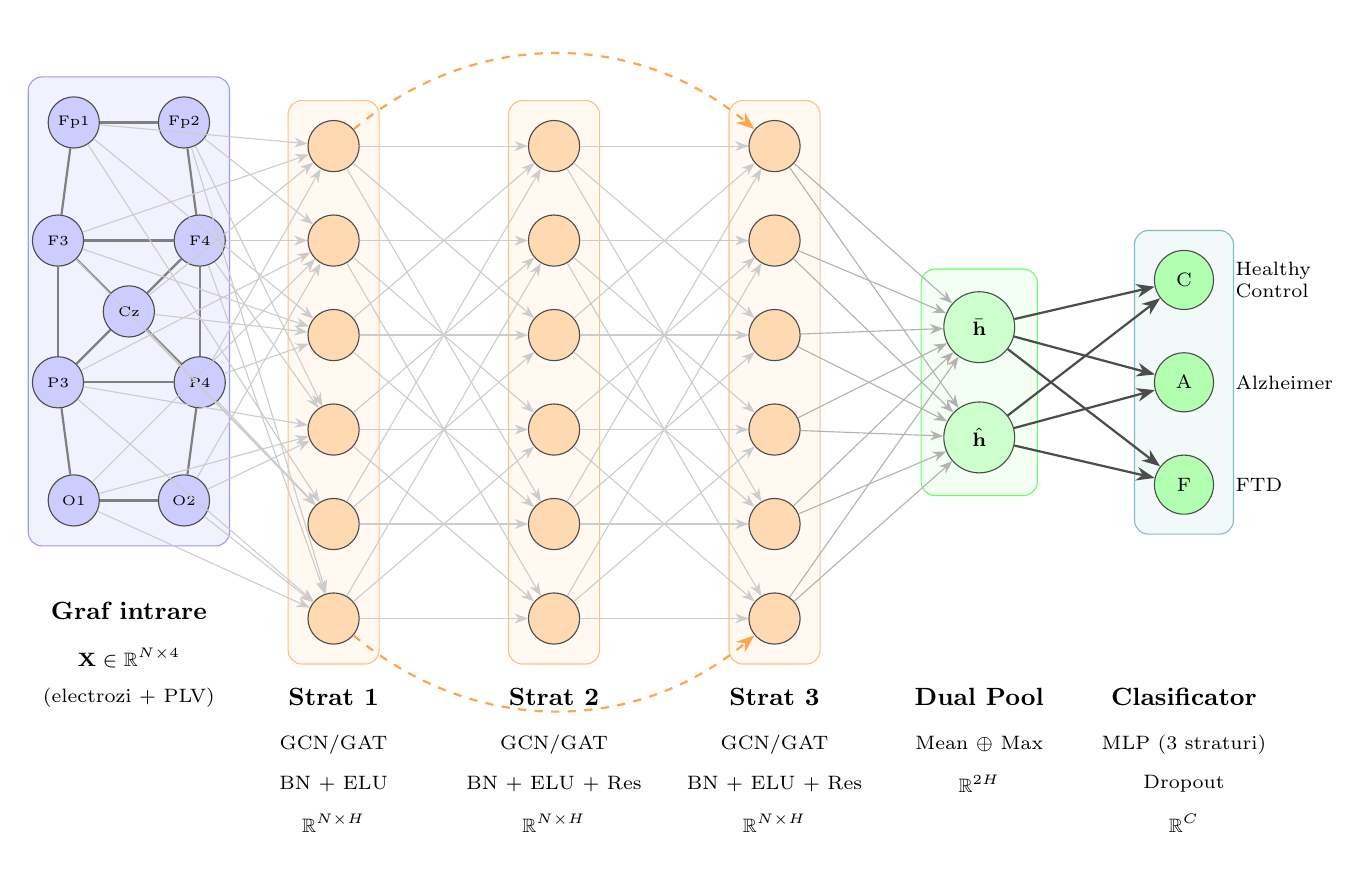
\begin{tikzpicture}[
    node/.style={circle, draw=black!70, fill=blue!20,
                 minimum size=0.65cm, inner sep=0pt, font=\tiny},
    hidnode/.style={circle, draw=black!70, fill=orange!30,
                    minimum size=0.65cm, inner sep=0pt},
    outnode/.style={circle, draw=black!70, fill=green!30,
                    minimum size=0.75cm, inner sep=0pt, font=\scriptsize},
    poolnode/.style={circle, draw=black!70, fill=green!20,
                     minimum size=0.9cm, inner sep=0pt, font=\scriptsize},
    conn/.style={->, gray!40, thin},
    resid/.style={->, dashed, orange!70, thick},
    >=Stealth
]

%% =========================================================
%% COLOANA 0 — Graf de intrare (electrozi) — dispunere 2D tip creier
%% =========================================================
\node[node] (n1) at (-0.5,  4.8) {Fp1};
\node[node] (n2) at ( 0.9,  4.8) {Fp2};
\node[node] (n3) at (-0.7,  3.3) {F3};
\node[node] (n4) at ( 1.1,  3.3) {F4};
\node[node] (n5) at ( 0.2,  2.4) {Cz};
\node[node] (n6) at (-0.7,  1.5) {P3};
\node[node] (n7) at ( 1.1,  1.5) {P4};
\node[node] (n8) at (-0.5,  0.0) {O1};
\node[node] (n9) at ( 0.9,  0.0) {O2};

% Muchii = conectivitate (PLV / topologică)
\draw[gray, thick] (n1)--(n2);
\draw[gray, thick] (n1)--(n3);
\draw[gray, thick] (n2)--(n4);
\draw[gray, thick] (n3)--(n4);
\draw[gray, thick] (n3)--(n5);
\draw[gray, thick] (n4)--(n5);
\draw[gray, thick] (n5)--(n6);
\draw[gray, thick] (n5)--(n7);
\draw[gray, thick] (n6)--(n7);
\draw[gray, thick] (n6)--(n8);
\draw[gray, thick] (n7)--(n9);
\draw[gray, thick] (n8)--(n9);
\draw[gray, thick] (n3)--(n6);
\draw[gray, thick] (n4)--(n7);

\node[align=center, font=\small]      at (0.2, -1.4) {\textbf{Graf intrare}};
\node[align=center, font=\scriptsize] at (0.2, -2.0) {$\mathbf{X} \in \mathbb{R}^{N \times 4}$};
\node[align=center, font=\scriptsize] at (0.2, -2.5) {(electrozi + PLV)};

%% =========================================================
%% COLOANA 1 — Strat GCN/GAT 1
%% =========================================================
\node[hidnode] (h1) at (2.8,  4.5) {};
\node[hidnode] (h2) at (2.8,  3.3) {};
\node[hidnode] (h3) at (2.8,  2.1) {};
\node[hidnode] (h4) at (2.8,  0.9) {};
\node[hidnode] (h5) at (2.8, -0.3) {};
\node[hidnode] (h6) at (2.8, -1.5) {};

\foreach \s in {n1,n3,n5,n7}
    \foreach \t in {h1,h3,h5}
        \draw[conn] (\s)--(\t);
\foreach \s in {n2,n4,n6,n8,n9}
    \foreach \t in {h2,h4,h6}
        \draw[conn] (\s)--(\t);

\node[align=center, font=\small]      at (2.8, -2.5) {\textbf{Strat 1}};
\node[align=center, font=\scriptsize] at (2.8, -3.1) {GCN/GAT};
\node[align=center, font=\scriptsize] at (2.8, -3.6) {BN + ELU};
\node[align=center, font=\scriptsize] at (2.8, -4.1) {$\mathbb{R}^{N \times H}$};

%% =========================================================
%% COLOANA 2 — Strat GCN/GAT 2 (+ residual din strat 1)
%% =========================================================
\node[hidnode] (g1) at (5.6,  4.5) {};
\node[hidnode] (g2) at (5.6,  3.3) {};
\node[hidnode] (g3) at (5.6,  2.1) {};
\node[hidnode] (g4) at (5.6,  0.9) {};
\node[hidnode] (g5) at (5.6, -0.3) {};
\node[hidnode] (g6) at (5.6, -1.5) {};

\foreach \s in {h1,h3,h5}
    \foreach \t in {g1,g3,g5}
        \draw[conn] (\s)--(\t);
\foreach \s in {h2,h4,h6}
    \foreach \t in {g2,g4,g6}
        \draw[conn] (\s)--(\t);

\node[align=center, font=\small]      at (5.6, -2.5) {\textbf{Strat 2}};
\node[align=center, font=\scriptsize] at (5.6, -3.1) {GCN/GAT};
\node[align=center, font=\scriptsize] at (5.6, -3.6) {BN + ELU + Res};
\node[align=center, font=\scriptsize] at (5.6, -4.1) {$\mathbb{R}^{N \times H}$};

%% =========================================================
%% COLOANA 3 — Strat GCN/GAT 3 (+ residual)
%% =========================================================
\node[hidnode] (f1) at (8.4,  4.5) {};
\node[hidnode] (f2) at (8.4,  3.3) {};
\node[hidnode] (f3) at (8.4,  2.1) {};
\node[hidnode] (f4) at (8.4,  0.9) {};
\node[hidnode] (f5) at (8.4, -0.3) {};
\node[hidnode] (f6) at (8.4, -1.5) {};

\foreach \s in {g1,g3,g5}
    \foreach \t in {f1,f3,f5}
        \draw[conn] (\s)--(\t);
\foreach \s in {g2,g4,g6}
    \foreach \t in {f2,f4,f6}
        \draw[conn] (\s)--(\t);

% Conexiuni reziduale (din strat 1 la strat 3, pe deasupra)
\draw[resid] (h1) to[bend left=40] (f1);
\draw[resid] (h6) to[bend right=40] (f6);

\node[align=center, font=\small]      at (8.4, -2.5) {\textbf{Strat 3}};
\node[align=center, font=\scriptsize] at (8.4, -3.1) {GCN/GAT};
\node[align=center, font=\scriptsize] at (8.4, -3.6) {BN + ELU + Res};
\node[align=center, font=\scriptsize] at (8.4, -4.1) {$\mathbb{R}^{N \times H}$};

%% =========================================================
%% COLOANA 4 — Dual Global Pooling (Mean + Max)
%% =========================================================
\node[poolnode] (pmean) at (11.0, 2.2) {$\bar{\mathbf{h}}$};
\node[poolnode] (pmax)  at (11.0, 0.8) {$\hat{\mathbf{h}}$};

\foreach \s in {f1,f2,f3,f4,f5,f6} {
    \draw[->, gray!60, thin] (\s)--(pmean);
    \draw[->, gray!60, thin] (\s)--(pmax);
}

\node[align=center, font=\small]      at (11.0, -2.5) {\textbf{Dual Pool}};
\node[align=center, font=\scriptsize] at (11.0, -3.1) {Mean $\oplus$ Max};
\node[align=center, font=\scriptsize] at (11.0, -3.6) {$\mathbb{R}^{2H}$};

%% =========================================================
%% COLOANA 5 — MLP Classifier
%% =========================================================
\node[outnode] (c1) at (13.6,  2.8) {C};
\node[outnode] (c2) at (13.6,  1.5) {A};
\node[outnode] (c3) at (13.6,  0.2) {F};

\draw[->, thick, black!70] (pmean)--(c1);
\draw[->, thick, black!70] (pmean)--(c2);
\draw[->, thick, black!70] (pmean)--(c3);
\draw[->, thick, black!70] (pmax)--(c1);
\draw[->, thick, black!70] (pmax)--(c2);
\draw[->, thick, black!70] (pmax)--(c3);

\node[right=0.15cm of c1, font=\scriptsize, align=left] {Healthy\\Control};
\node[right=0.15cm of c2, font=\scriptsize, align=left] {Alzheimer};
\node[right=0.15cm of c3, font=\scriptsize, align=left] {FTD};

\node[align=center, font=\small]      at (13.6, -2.5) {\textbf{Clasificator}};
\node[align=center, font=\scriptsize] at (13.6, -3.1) {MLP (3 straturi)};
\node[align=center, font=\scriptsize] at (13.6, -3.6) {Dropout};
\node[align=center, font=\scriptsize] at (13.6, -4.1) {$\mathbb{R}^{C}$};

%% =========================================================
%% Dreptunghiuri de grupare (background)
%% =========================================================
\begin{scope}[on background layer]
    \node[draw=blue!40, fill=blue!5, rounded corners=5pt, fit=(n1)(n2)(n8)(n9), inner sep=7pt] {};
    \node[draw=orange!50, fill=orange!5, rounded corners=5pt, fit=(h1)(h6), inner sep=7pt] {};
    \node[draw=orange!50, fill=orange!5, rounded corners=5pt, fit=(g1)(g6), inner sep=7pt] {};
    \node[draw=orange!50, fill=orange!5, rounded corners=5pt, fit=(f1)(f6), inner sep=7pt] {};
    \node[draw=green!60,  fill=green!5,  rounded corners=5pt, fit=(pmean)(pmax), inner sep=8pt] {};
    \node[draw=teal!50,   fill=teal!5,   rounded corners=5pt, fit=(c1)(c3), inner sep=7pt] {};
\end{scope}

\end{tikzpicture}
\caption{Arhitectura rețelei neuronale de tip graf (GCN/GAT) utilizate pentru clasificarea
semnalelor EEG: graful de intrare cu electrozi și conectivitate ponderată, trei straturi de
propagare cu normalizare batch, activare ELU și conexiuni reziduale, agregare globală prin
concatenarea mediei și maximului (\textit{dual pooling}), și clasificator MLP cu trei straturi
liniare. Săgețile portocalii punctate reprezintă conexiunile reziduale (\textit{skip connections}).}
\label{fig:gnn_architecture}
\end{figure}

\section{Procesarea semnalelor EEG utilizând rețele neuronale de tip graf}

În ultimii ani, utilizarea rețelelor neuronale de tip graf (Graph Neural Networks - GNN) în analiza semnalelor EEG a cunoscut o creștere semnificativă, datorită capacității acestora de a modela relațiile complexe dintre diferitele regiuni ale creierului. Spre deosebire de metodele tradiționale, care tratează canalele EEG independent sau presupun relații locale fixe, abordările bazate pe grafuri permit captarea interdependenței funcționale și structurale dintre electrozi, oferind o reprezentare mai fidelă a activității cerebrale \cite{klepl2023gnn}.

Un aspect central al acestor metode îl reprezintă modul în care este construit graful asociat datelor EEG. În majoritatea lucrărilor, electrozii sunt modelați ca noduri, iar muchiile sunt definite fie pe baza distanței fizice dintre electrozi, fie pe baza unor măsuri de conectivitate funcțională, precum corelația sau coerența semnalelor. Această flexibilitate permite adaptarea structurii grafului în funcție de aplicație și de natura datelor analizate \cite{rahman2025advancement}.

Numeroase studii au demonstrat eficiența utilizării modelelor GNN în diverse sarcini legate de procesarea semnalelor EEG, precum clasificarea stărilor cognitive, detecția crizelor epileptice sau identificarea afecțiunilor neurologice și neurodegenerative. De exemplu, în contextul detecției epilepsiei, modelele GNN au fost utilizate pentru a surprinde tiparele spațio-temporale ale activității cerebrale, obținând performanțe superioare față de metodele clasice de învățare automată \cite{awais2024graphical}.

Un domeniu deosebit de important în care rețelele neuronale graf au demonstrat un potențial ridicat este diagnosticarea și analiza bolilor neurodegenerative, în special a bolii Alzheimer. Această afecțiune este caracterizată prin modificări subtile ale activității cerebrale, care pot fi dificil de detectat prin metode tradiționale. Utilizarea GNN permite modelarea rețelelor funcționale ale creierului și identificarea unor tipare specifice asociate declinului cognitiv.

În acest context, studiul realizat de Hu et al. \cite{hu2024self} propune un model de rețea neuronală graf explicabilă pentru predicția riscului asociat bolii Alzheimer și demențelor înrudite, demonstrând potențialul acestor modele în aplicații biomedicale cu componentă de interpretabilitate. Această caracteristică este deosebit de importantă în aplicațiile medicale, unde încrederea în model și capacitatea de a explica deciziile sunt esențiale pentru adoptarea pe scară largă a acestor tehnologii.

Pe lângă modelele GCN, care oferă o agregare eficientă a informației, lucrările recente evidențiază avantajele utilizării mecanismelor de atenție, precum în cazul modelelor GAT. Acestea permit identificarea conexiunilor relevante dintre regiuni cerebrale și adaptarea dinamică a ponderilor asociate muchiilor, ceea ce este esențial în analiza datelor EEG, unde relațiile dintre canale pot varia în timp și în funcție de sarcina analizată \cite{klepl2023gnn,rahman2025advancement}.

În general, abordările bazate pe GNN oferă un cadru unificat pentru integrarea informațiilor spațiale și temporale din semnalele EEG. Prin modelarea explicită a relațiilor dintre electrozi, aceste metode reușesc să captureze structura complexă a activității cerebrale și să îmbunătățească performanța în sarcini de clasificare și detecție.

Cu toate acestea, există și provocări asociate utilizării GNN în acest domeniu. Printre acestea se numără alegerea optimă a structurii grafului, scalabilitatea modelelor și necesitatea unor seturi de date bine etichetate. În plus, variabilitatea ridicată a semnalelor EEG între subiecți poate afecta capacitatea de generalizare a modelelor.

În concluzie, rețelele neuronale de tip graf reprezintă o direcție promițătoare în analiza semnalelor EEG, oferind avantaje semnificative față de metodele tradiționale. Capacitatea acestora de a modela relațiile complexe dintre regiunile cerebrale le face deosebit de potrivite pentru aplicații în domeniul biomedical, inclusiv pentru detectarea și monitorizarea bolilor neurodegenerative precum Alzheimer. 

\chapter{Implementare}

În cadrul acestui capitol este descris în detaliu procesul de implementare al întregului pipeline propus pentru analiza și clasificarea semnalelor EEG utilizând rețele neuronale de tip graf. Sunt prezentate setul de date utilizat, etapele concrete de pre-procesare, construirea reprezentărilor de tip graf, arhitecturile modelelor implementate, procesul de antrenare și mecanismul de inferență. Implementarea a fost realizată în limbajul Python, utilizând bibliotecile MNE \cite{gramfort2013mne} pentru procesarea semnalelor EEG și PyTorch Geometric \cite{fey2019fast} pentru construirea și antrenarea modelelor de rețele neuronale graf.

\section{Setul de date utilizat}

Setul de date utilizat în cadrul prezentei lucrări conține înregistrări EEG provenite de la subiecți din trei categorii clinice: persoane sănătoase (Healthy Control -- C), pacienți diagnosticați cu boala Alzheimer (A) și pacienți diagnosticați cu demență frontotemporală (F).\footnote{Setul de date este disponibil public la adresa: \url{https://openneuro.org/datasets/ds004504}.} Înregistrările corespund protocolului experimental \textit{eyes closed}, în care subiecții sunt monitorizați în stare de repaus cu ochii închiși, protocol frecvent utilizat în studiile privind afecțiunile neurodegenerative.

\subsection{Formatul și structura datelor}
\label{sec:format_date}

Fișierele EEG sunt stocate în formatul EEGLAB \texttt{.set}, un format standard utilizat pe scară largă în comunitatea de cercetare în neuroștiințe. Structura directoarelor urmează convenția BIDS (Brain Imaging Data Structure), fiecare subiect având un director dedicat care conține înregistrarea EEG corespunzătoare:

\begin{verbatim}
data/
|-- participants_train.tsv
|-- derivatives/
|   |-- sub-001/
|   |   +-- eeg/
|   |       +-- sub-001_task-eyesclosed_eeg.set
|   |-- sub-002/
|   |   +-- eeg/
|   |       +-- sub-002_task-eyesclosed_eeg.set
|   +-- ...
+-- holdout_diagnosis/
    |-- sub-024/
    |   +-- eeg/
    |       +-- sub-024_task-eyesclosed_eeg.set
    +-- ...
\end{verbatim}

Fișierul \texttt{participants\_train.tsv} conține metadatele asociate fiecărui subiect, incluzând identificatorul unic (\texttt{participant\_id}) și grupul clinic (\texttt{Group}). Acest fișier este utilizat pentru a asocia fiecărei înregistrări EEG eticheta corespunzătoare în procesul de construire a setului de date pentru antrenare.

Directorul \texttt{holdout\_diagnosis/} conține înregistrări EEG rezervate exclusiv pentru etapa de inferență și testare finală, aceste date nefiind utilizate în procesul de antrenare sau validare a modelelor.

\subsection{Configurația claselor de clasificare}

Sistemul implementat suportă două moduri de clasificare, configurabile de către utilizator:

\begin{itemize}
    \item \textbf{Clasificare binară} -- în care sunt utilizate doar grupurile C (Healthy Control) și A (Alzheimer's Disease), subiecții din grupul F fiind excluși. Etichetele asociate sunt: 0 pentru clasa C și 1 pentru clasa A.
    \item \textbf{Clasificare pe trei clase} -- în care sunt utilizate toate cele trei grupuri: C, A și F (Frontotemporal Dementia). Etichetele asociate sunt: 0 pentru C, 1 pentru A și 2 pentru F.
\end{itemize}

Această flexibilitate permite evaluarea modelelor atât în scenariul simplificat de diferențiere între starea sănătoasă și boala Alzheimer, cât și în scenariul mai complex de clasificare a trei tipuri distincte de stări cognitive. Maparea dintre grupurile clinice și etichetele numerice este centralizată într-un dicționar de configurare, asigurând consistența pe tot parcursul pipeline-ului.

\subsection{Selecția canalelor EEG}
\label{sec:canal_selectie}

Din totalul canalelor disponibile în fiecare înregistrare, sunt reținute doar cele 19 canale corespunzătoare sistemului internațional de plasare a electrozilor 10-20, un standard utilizat pe scară largă în electroencefalografia clinică și de cercetare. Canalele selectate sunt: Fp1, Fp2, F7, F3, Fz, F4, F8, T3, C3, Cz, C4, T4, T5, P3, Pz, P4, T6, O1 și O2.

Această selecție asigură o acoperire uniformă a regiunilor cerebrale (frontală, centrală, temporală, parietală și occipitală) și garantează compatibilitatea între înregistrările provenite de la diferiți subiecți, eliminând eventualele canale suplimentare sau specifice anumitor configurații de echipamente.

% ============================================================
% SECTIUNEA 3.2 — PRE-PROCESAREA SEMNALELOR EEG
% ============================================================
\section{Pre-procesarea semnalelor EEG}
\label{sec:impl_preprocesare}

Etapa de pre-procesare reprezintă primul pas operațional în pipeline-ul implementat și are rolul de a transforma înregistrările EEG brute în date curate și structurate, potrivite pentru extragerea caracteristicilor și construirea ulterioară a reprezentărilor de tip graf. Întreaga logică de pre-procesare este implementată în modulul \texttt{src/preprocessing.py}, utilizând biblioteca MNE \cite{gramfort2013mne}. Pașii principali ai acestui modul sunt ilustrați în ordinea lor de execuție: încărcarea fișierului, selecția canalelor, filtrarea, curățarea opțională prin ICA, segmentarea în ferestre de timp și conversia la format NumPy.

\subsection{Încărcarea fișierelor EEG}

Fișierele EEG în format EEGLAB \texttt{.set} sunt încărcate prin intermediul
funcției \texttt{mne.io.read\_raw\_eeglab()} din biblioteca MNE\@, cu parametrul
\texttt{preload=True}, care determină încărcarea completă a datelor în memoria RAM în momentul citirii. Rezultatul este un obiect de tip \texttt{mne.io.BaseRaw}, care încapsulează atât datele brute ale semnalului, cât și metadatele asociate înregistrării: rata de eșantionare $f_s$, lista denumirilor canalelor, durata totală a înregistrării și informații despre sistemul de achiziție.

Verificarea existenței fizice a fișierului pe disc este realizată anterior apelului de citire, generând o excepție explicită (\texttt{FileNotFoundError}) în cazul în care fișierul nu poate fi localizat. Această validare preventivă asigură un comportament robust al pipeline-ului în cazul unor seturi de date incomplete sau al unor erori de configurare a căilor de acces.

\subsection{Filtrarea trece-bandă}

După încărcare și selecția canalelor standard (descrisă în Secțiunea~\ref{sec:canal_selectie}), semnalul este supus unui proces de filtrare trece-bandă, cu scopul de a elimina componentele spectrale irelevante sau perturbatoare și de a păstra exclusiv banda de frecvență de interes pentru analiza activității cerebrale.

Se aplică un filtru FIR (Finite Impulse Response) de tip \textit{firwin} (fereastră Hanning), cu frecvența inferioară $f_l = 0.5$~Hz și frecvența superioară $f_h = 45.0$~Hz, prin intermediul metodei \texttt{raw.filter(l\_freq, h\_freq, fir\_design=\textquotedbl firwin\textquotedbl)} din biblioteca MNE.

Alegerea acestor limite de frecvență este motivată fiziologic și tehnic:
\begin{itemize}
    \item Frecvența inferioară $f_l = 0.5$~Hz elimină componenta de curent continuu (DC offset) și deriva lentă a liniei de bază (baseline drift), care pot apărea datorită mișcărilor subiectului sau impedanței variabile a electrozilor;
    \item Frecvența superioară $f_h = 45.0$~Hz elimină artefactele de înaltă frecvență și interferențele de la rețeaua electrică (50~Hz în Europa), fără a afecta benzile de interes clinic (Delta, Theta, Alpha, Beta -- toate sub 30~Hz).
\end{itemize}

Filtrul FIR a fost ales față de alternativa IIR (Infinite Impulse Response) deoarece garantează o \textbf{fază liniară}: toate componentele frecvențiale ale semnalului sunt întârziate cu același interval de timp, fără distorsiuni de fază. Această proprietate este esențială în analiza semnalelor EEG, unde relațiile de fază dintre canale constituie baza calculului PLV descris în Secțiunea~\ref{sec:plv} \cite{awais2024graphical,rahman2025advancement}.

\subsection{Curățarea prin ICA}
\label{sec:ica}

Opțional, după filtrare, poate fi aplicat un pas de curățare a artefactelor prin Analiza Componentelor Independente (Independent Component Analysis -- ICA). Această etapă este controlată prin parametrul boolean \texttt{apply\_ica} al funcției principale de pre-procesare și este dezactivată implicit (\texttt{apply\_ica=False}).

Algoritmul ICA descompune semnalul EEG multicanal într-un set de componente statistice independente. Formal, fie $\mathbf{X} \in \mathbb{R}^{N_c \times T}$ matricea semnalului EEG, cu $N_c$ canale și $T$ eșantioane temporale. ICA caută o matrice de mixare $\mathbf{M}$ și sursele independente $\mathbf{S}$, astfel încât:
\begin{equation}
    \mathbf{X} = \mathbf{M} \cdot \mathbf{S}
    \label{eq:ica}
\end{equation}

\noindent unde:
\begin{itemize}
    \item $\mathbf{X} \in \mathbb{R}^{N_c \times T}$ -- matricea semnalului EEG observat;
    \item $\mathbf{M} \in \mathbb{R}^{N_c \times n}$ -- matricea de mixare (mixing matrix), cu $n$ numărul de componente independente;
    \item $\mathbf{S} \in \mathbb{R}^{n \times T}$ -- matricea surselor independente estimate.
\end{itemize}

Componentele asociate artefactelor tipice (clipit, mișcări oculare, activitate musculară) au, în general, o formă caracteristică în spațiul surselor și pot fi identificate și eliminate, iar semnalul este reconstruit din componentele rămase. Numărul de componente ICA este setat la $n = \min(15, N_c)$, iar starea inițială a algoritmului este fixată prin \texttt{random\_state = 42} pentru a asigura reproductibilitatea rezultatelor.

Etapa ICA este lăsată opțională deoarece, în absența unei inspecții manuale a componentelor, există riscul eliminării unor componente cerebrale relevante. Acest aspect este cu atât mai important în contextul seturilor de date de cercetare clinică, unde minimizarea pierderii de informație este prioritară \cite{awais2024graphical,rahman2025advancement}.

\subsection{Segmentarea în epoci}

Semnalul continuu, după filtrare și curățare, este segmentat în ferestre de timp de lungime fixă printr-un proces denumit \textit{epoching}. Această etapă transformă înregistrarea continuă într-o colecție de segmente independente, fiecare urmând a fi procesat ca o instanță separată în pipeline-ul de construire a grafurilor.

În implementarea de față, fiecare epocă are durata $\Delta t = 5$~secunde, fără suprapunere ($\text{overlap} = 0$~s). Evenimentele de segmentare sunt generate automat cu funcția \texttt{mne.make\_fixed\_length\_events()}, iar obiectul \texttt{mne.Epochs} este construit cu parametrul \texttt{detrend=1}, care aplică o eliminare liniară a tendinței (\textit{linear detrending}) pentru fiecare epocă în parte.

Detrending-ul liniar elimină tendința de primă ordine din fiecare epocă: se ajustează un polinom de gradul 1 pe datele epocii și se scade din semnal, prevenind astfel influența variațiilor lente de nivel (low-frequency drift) asupra caracteristicilor spectrale extrase ulterior.

Numărul de epoci $N_e$ obținute dintr-o înregistrare de durată totală $D$ secunde este aproximat prin:
\begin{equation}
    N_e = \left\lfloor \frac{D}{\Delta t} \right\rfloor
    \label{eq:num_epochs}
\end{equation}

\noindent unde:
\begin{itemize}
    \item $N_e$ -- numărul de epoci extrase;
    \item $D$ -- durata totală a înregistrării EEG (secunde);
    \item $\Delta t = 5$~s -- durata unei epoci;
    \item $\lfloor \cdot \rfloor$ -- partea întreagă inferioară (floor).
\end{itemize}

Fiecare epocă rezultată este tratată ca o instanță independentă de antrenare, ceea ce multiplică semnificativ numărul de exemple disponibile per subiect și contribuie la creșterea diversității datelor de antrenare. Această alegere este standard în literatura de specialitate pentru clasificarea semnalelor EEG în stare de repaus \cite{klepl2023gnn,awais2024graphical}.

\subsection{Conversia la format NumPy}

În ultima etapă a modulului de pre-procesare, epocile sunt convertite dintr-un obiect \texttt{mne.Epochs} într-un array NumPy tridimensional, utilizând metoda \texttt{epochs.get\_data()}. Array-ul rezultat are forma:
\begin{equation}
    \mathbf{X} \in \mathbb{R}^{N_e \times N_c \times N_t}
    \label{eq:epoch_array}
\end{equation}

\noindent unde:
\begin{itemize}
    \item $N_e$ -- numărul de epoci extrase din înregistrare;
    \item $N_c = 19$ -- numărul de canale EEG, conform selecției sistemului 10-20;
    \item $N_t = \Delta t \cdot f_s$ -- numărul de eșantioane temporale per epocă, determinat de durata epocii $\Delta t$ și rata de eșantionare $f_s$ a înregistrării.
\end{itemize}

Valorile din array sunt exprimate în volți (unitatea nativă a obiectului MNE). Conversia la microvol\-ți ($\mu V$) este realizată ulterior, în modulul de construire a grafurilor, prin înmulțire cu factorul $10^6$, facilitând scalarea numerică adecvată pentru calculul densității spectrale de putere.

Acest tensor tridimensional $\mathbf{X}$ constituie ieșirea modulului de pre-procesare și intrarea directă pentru modulul de construire a grafurilor, descris în secțiunea următoare.

\begin{figure}[H]
    \centering
    \begin{minipage}{0.48\textwidth}
        \centering
        \includegraphics[width=\textwidth]{images/EEG_Before.png}
        \caption{(a) Înainte de pre-procesare}
    \end{minipage}
    \hfill
    \begin{minipage}{0.48\textwidth}
        \centering
        \includegraphics[width=\textwidth]{images/EEG_After.png}
        \caption{(b) După pre-procesare}
    \end{minipage}
    \caption{Semnalul EEG înainte și după etapa de pre-procesare.}
    \label{fig:preprocesare}
\end{figure}

% ============================================================
% SECTIUNEA 3.3 — CONSTRUIREA REPREZENTARILOR DE TIP GRAF
% ============================================================
\section{Construirea reprezentărilor de tip graf}
\label{sec:impl_graf}

Odată ce semnalele EEG au fost pre-procesate și convertite în tensorul de epoci $\mathbf{X} \in \mathbb{R}^{N_e \times N_c \times N_t}$, fiecare epocă este transformată individual într-un graf compatibil cu biblioteca PyTorch Geometric. Această etapă este implementată în modulul \texttt{src/graph\_builder.py} și cuprinde trei operații principale: extragerea trăsăturilor nodurilor, calculul matricei de conectivitate funcțională prin PLV și conversia la formatul intern al obiectului \texttt{Data} din PyG.

\subsection{Extragerea trăsăturilor nodurilor}

Fiecare nod al grafului corespunde unui electrod EEG și este caracterizat printr-un vector de trăsături care codifică informația spectrală a semnalului înregistrat de acel electrod în cadrul epocii respective. Trăsăturile sunt calculate ca puterea medie a semnalului pe cele patru benzi de frecvență standard: Delta ($\delta$: 0.5--4~Hz), Theta ($\theta$: 4--8~Hz), Alpha ($\alpha$: 8--12~Hz) și Beta ($\beta$: 12--30~Hz), conform Tabelului~\ref{tab:eeg_bands}.

Calculul puterii spectrale se realizează prin metoda Welch \cite{awais2024graphical}, care estimează densitatea spectrală de putere (PSD) prin medierea periodogramelor calculate pe segmente suprapuse ale semnalului. Pentru canalul $c$ și banda de frecvență $[f_l, f_h]$, puterea medie este:
\begin{equation}
    P_c^{[f_l, f_h]} = \frac{1}{|\mathcal{F}_{[f_l,f_h]}|} \sum_{f \in \mathcal{F}_{[f_l,f_h]}} \widehat{S}_c(f)
    \label{eq:band_power}
\end{equation}

\noindent unde:
\begin{itemize}
    \item $P_c^{[f_l, f_h]}$ -- puterea medie a canalului $c$ în banda $[f_l, f_h]$;
    \item $\mathcal{F}_{[f_l,f_h]}$ -- mulțimea bin-urilor de frecvență ale PSD care se încadrează în intervalul $[f_l, f_h]$;
    \item $\widehat{S}_c(f)$ -- estimatul PSD al canalului $c$ la frecvența $f$, obținut prin metoda Welch;
    \item $|\mathcal{F}_{[f_l,f_h]}|$ -- numărul de bin-uri de frecvență din bandă.
\end{itemize}

Lungimea segmentului utilizat de metoda Welch este $n_{seg} = \min(2 f_s, N_t)$ eșantioane, unde $f_s$ este rata de eșantionare și $N_t$ este numărul de eșantioane ale epocii. Această alegere asigură o rezoluție spectrală de cel puțin 0.5~Hz, suficientă pentru delimitarea benzilor de interes. Datele sunt în prealabil convertite la microvol\-ți ($\mu V$) prin înmulțire cu factorul $10^6$, facilitând o scalare numerică adecvată.

Rezultatul este matricea de trăsături ale nodurilor:
\begin{equation}
    \mathbf{X}_{nod} \in \mathbb{R}^{N_c \times 4}
    \label{eq:node_features}
\end{equation}

\noindent unde fiecare linie $c \in \{1, \ldots, N_c\}$ conține vectorul $[P_c^{\delta},\, P_c^{\theta},\, P_c^{\alpha},\, P_c^{\beta}]$ al puterii medii pe cele patru benzi. Cu $N_c = 19$ canale, fiecare nod este descris printr-un vector de dimensiune 4.

Alegerea puterii spectrale pe benzi ca trăsături ale nodurilor este motivată de relevanța fiziologică a acestor benzi în contextul afecțiunilor neurodegenerative, discutată în Secțiunea~\ref{sec:benzi}, și de caracterul lor compact și interpretabil, care facilitează atât antrenarea, cât și analiza ulterioară a modelului.

\subsection{Calculul matricei de conectivitate funcțională}

Muchiile grafului sunt definite pe baza sincronizării funcționale dintre perechi de electrozi, cuantificată prin Phase Locking Value (PLV), introdus teoretic în Secțiunea~\ref{sec:plv}. Calculul PLV este aplicat în banda Alpha (8--12~Hz), motivat de relevanta acestei benzi în detectarea modificărilor asociate bolii Alzheimer, unde reducerea activității alpha constituie un biomarker clinic important \cite{klepl2023gnn}.

Procesul de calcul pentru o epocă $\mathbf{e} \in \mathbb{R}^{N_c \times N_t}$ urmează trei pași:

\textbf{Pasul 1 — Filtrare în bandă.} Semnalul fiecărui canal este filtrat în banda Alpha printr-un filtru Butterworth trece-bandă de ordinul 4, implementat cu filtrare bidirecțională (\texttt{filtfilt}) pentru a elimina distorsiunile de fază:
\begin{equation}
    \tilde{e}_c(t) = \text{filtfilt}_{[8, 12]\,\text{Hz}}\left(e_c(t)\right), \quad c = 1, \ldots, N_c
    \label{eq:butter_filter}
\end{equation}

\noindent Filtrarea bidirecțională aplică filtrul de două ori — o dată înainte și o dată înapoi în timp — rezultând o fază zero netă și o atenuare dublă față de un singur pas de filtrare.

\textbf{Pasul 2 — Extragerea fazei instantanee.} Se aplică transformata Hilbert semnalelor filtrate pentru a obține fazele instantanee, conform ecuațiilor~\eqref{eq:analytic} și~\eqref{eq:instantaneous_phase}:
\begin{equation}
    \phi_c(t) = \arg\!\left(\tilde{e}_c(t) + i \cdot \mathcal{H}[\tilde{e}_c(t)]\right), \quad c = 1, \ldots, N_c
    \label{eq:phase_extraction}
\end{equation}

\textbf{Pasul 3 — Calculul PLV pentru toate perechile.} PLV se calculează pentru fiecare pereche $(i, j)$ cu $i < j$, conform ecuației~\eqref{eq:plv}, și se completează simetric:
\begin{equation}
    \mathbf{PLV} \in \mathbb{R}^{N_c \times N_c}, \quad \mathbf{PLV}_{ij} = \mathbf{PLV}_{ji}, \quad \mathbf{PLV}_{ii} = 0
    \label{eq:plv_matrix}
\end{equation}

Diagonala principală este setată la zero pentru a evita auto-conexiunile nodurilor. Matricea $\mathbf{PLV}$ constituie matricea de adiacență ponderată brută a grafului.

\subsection{Aplicarea pragului de adiacență}

Matricea PLV completă conține valori nenule pentru toate perechile de electrozi, ceea ce ar conduce la un graf dens, cu $N_c(N_c-1)$ muchii direcționate, respectiv $\frac{N_c(N_c-1)}{2}$ muchii nedirecționate. Un graf prea dens poate introduce zgomot structural și poate îngreuna procesul de învățare al modelului GNN, deoarece conexiunile cu sincronizare funcțională slabă nu transmit informație relevantă \cite{rahman2025advancement}.

Pentru a obține un graf mai sparse și semnificativ din punct de vedere funcțional, se aplică un prag $\tau \in [0, 1]$ asupra matricei PLV:
\begin{equation}
    \mathbf{A}_{ij} =
    \begin{cases}
        \mathbf{PLV}_{ij} & \text{dacă } \mathbf{PLV}_{ij} \geq \tau \\
        0 & \text{altfel}
    \end{cases}
    \label{eq:threshold}
\end{equation}

\noindent unde:
\begin{itemize}
    \item $\mathbf{A} \in \mathbb{R}^{N_c \times N_c}$ -- matricea de adiacență ponderată a grafului, după aplicarea pragului;
    \item $\tau$ -- pragul de conectivitate, parametru configurabil de către utilizator;
    \item valorile sub $\tau$ sunt setate la zero, eliminând muchiile cu sincronizare slabă.
\end{itemize}

În implementarea prezentă, valoarea implicită a pragului este $\tau = 0.9$, reținând astfel doar conexiunile cu un grad ridicat de sincronizare de fază. Alegerea unui prag ridicat este motivată de natura setului de date utilizat (înregistrări în repaus cu ochii închiși), în care conectivitatea funcțională relevantă clinic este, în general, caracterizată prin valori PLV ridicate \cite{klepl2023gnn}. Pragul este totuși un hiperparametru configurabil, al cărui impact asupra performanței modelului este analizat în Capitolul~5.

\subsection{Conversia la formatul PyTorch Geometric}

Matricea de adiacență $\mathbf{A}$ este convertită la reprezentarea internă utilizată de PyTorch Geometric, care stochează grafurile în format \textit{sparse} prin două tensori:

\begin{itemize}
    \item \texttt{edge\_index} $\in \mathbb{Z}^{2 \times |\mathcal{E}|}$ -- tensorii de indici ai muchiilor, unde prima linie conține indicii nodurilor sursă, iar a doua linie indicii nodurilor destinație; $|\mathcal{E}|$ este numărul total de muchii după pragare;
    \item \texttt{edge\_attr} $\in \mathbb{R}^{|\mathcal{E}| \times 1}$ -- tensorul atributelor muchiilor, conținând valoarea PLV corespunzătoare fiecărei muchii.
\end{itemize}

Conversia se realizează prin identificarea pozițiilor nenule din $\mathbf{A}$ cu \texttt{numpy.nonzero()}, extragerea valorilor corespunzătoare și construirea tensorilor PyTorch cu tipurile de date corespunzătoare (\texttt{torch.long} pentru indici și \texttt{torch.float32} pentru atribute).

\subsection{Construirea obiectului \texttt{Data}}

Toate componentele calculate sunt asamblate într-un obiect de tip \texttt{Data} din biblioteca \texttt{torch\_geometric}, care reprezintă graful complet asociat unei epoci EEG:

\begin{equation}
    \mathcal{G} = \left(\mathbf{X}_{nod},\; \texttt{edge\_index},\; \texttt{edge\_attr},\; y,\; \texttt{subject\_id},\; \texttt{epoch\_index}\right)
    \label{eq:pyg_data}
\end{equation}

\noindent unde:
\begin{itemize}
    \item $\mathbf{X}_{nod} \in \mathbb{R}^{19 \times 4}$ -- matricea trăsăturilor nodurilor (puterea spectrală pe 4 benzi);
    \item \texttt{edge\_index} $\in \mathbb{Z}^{2 \times |\mathcal{E}|}$ -- conectivitatea grafului în format COO (Coordinate format);
    \item \texttt{edge\_attr} $\in \mathbb{R}^{|\mathcal{E}| \times 1}$ -- valorile PLV ale muchiilor;
    \item $y \in \{0, 1\}$ sau $y \in \{0, 1, 2\}$ -- eticheta clinică a subiectului (Healthy Control, Alzheimer, Frontotemporal Dementia);
    \item \texttt{subject\_id} -- identificatorul subiectului de origine, utilizat pentru split-ul subiect-nivel la antrenare;
    \item \texttt{epoch\_index} -- indexul ferestrei temporale în cadrul înregistrării subiectului.
\end{itemize}

Prin parcurgerea tuturor ferestrelor temporale ale tuturor subiectilor incluși în setul de date, se construiește o listă de obiecte \texttt{Data}, câte unul per fereastră, care constituie dataset-ul final utilizat la antrenare. Procesul de construire a acestui dataset este orchestrat de modulul \texttt{src/dataset\_builder.py}, descris în secțiunea următoare.

% ============================================================
% SECTIUNEA 3.4 — PREGĂTIREA SETULUI DE DATE PENTRU ANTRENARE
% ============================================================
\section{Pregătirea setului de date pentru antrenare}
\label{sec:dataset_builder}

Modulul \texttt{src/dataset\_builder.py} orchestrează întregul flux de construire a setului de date, de la citirea metadatelor clinice până la salvarea colecției finale de grafuri PyG pe disc. Acesta integrează secvențial operațiile descrise în Secțiunile~\ref{sec:impl_preprocesare} și~\ref{sec:impl_graf}, aplicându-le pentru fiecare subiect inclus în setul de antrenare.

\subsection{Citirea metadatelor și maparea etichetelor}

Punctul de intrare al procesului îl constituie fișierul \texttt{participants\_train.tsv}, care este citit ca un tabel structurat cu ajutorul bibliotecii \texttt{pandas}. Fiecare rând al tabelului conține identificatorul unui subiect (\texttt{participant\_id}) și grupul clinic din care face parte (\texttt{Group}).

Înainte de procesare, tabelul este validat pentru a asigura prezența coloanelor obligatorii. Grupul clinic al fiecărui subiect este normalizat la majuscule și comparat cu mulțimea grupurilor active pentru modul de clasificare selectat. Subiecții care aparțin unor grupuri excluse din configurația curentă sunt omisi fără a genera erori, iar motivul omiterii este jurnalizat explicit. Maparea dintre grupurile clinice și etichetele numerice utilizate la antrenare este centralizată în dicționarul de configurare prezentat în Tabelul~\ref{tab:label_mapping}.

\begin{table}[H]
    \centering
    \caption{Maparea grupurilor clinice la etichete numerice în funcție de modul de clasificare.}
    \label{tab:label_mapping}
    \begin{tabular}{|l|c|c|}
        \hline
        \textbf{Grup clinic} & \textbf{Etichetă (binar)} & \textbf{Etichetă (trei clase)} \\
        \hline
        C -- Healthy Control & 0 & 0 \\
        \hline
        A -- Alzheimer's Disease & 1 & 1 \\
        \hline
        F -- Frontotemporal Dementia & exclus & 2 \\
        \hline
    \end{tabular}
\end{table}

\subsection{Procesarea per subiect}

Pentru fiecare subiect inclus, pipeline-ul execută secvențial următoarele operații:

\begin{enumerate}
    \item \textbf{Localizarea fișierului EEG} -- calea fișierului este construită după convenția BIDS, prezentată în Secțiunea~\ref{sec:format_date}. Dacă fișierul nu există pe disc, subiectul este omis și evenimentul este jurnalizat;
    \item \textbf{Pre-procesarea semnalului} -- se apelează funcția \texttt{load\_and\_preprocess\_eeg()} din modulul \texttt{src/preprocessing.py}, care aplică secvența completă descrisă în Secțiunea~\ref{sec:impl_preprocesare}: încărcare, selecție canale, filtrare FIR și, opțional, curățare ICA;
    \item \textbf{Segmentarea în epoci} -- semnalul pre-procesat este segmentat în epoci de $\Delta t = 5$~s fără suprapunere, obținând tensorul $\mathbf{X} \in \mathbb{R}^{N_e \times 19 \times N_t}$;
    \item \textbf{Construirea grafurilor} -- pentru fiecare dintre cele $N_e$ epoci se construiește câte un obiect \texttt{Data} conform procedurii descrise în Secțiunea~\ref{sec:impl_graf}, utilizând pragul PLV configurat. Fiecare graf primește eticheta clinică a subiectului și identificatorul acestuia ca metadate;
    \item \textbf{Agregarea grafurilor} -- grafurile generate pentru subiectul curent sunt adăugate la lista globală a setului de date.
\end{enumerate}

În cazul în care procesarea unui subiect eșuează din motive tehnice (fișier corupt, număr insuficient de canale etc.), eroarea este capturată, motivul este jurnalizat, iar pipeline-ul continuă cu următorul subiect, fără a întrerupe procesarea întregului set de date.

\subsection{Raportarea statisticilor și salvarea pe disc}

La finalizarea procesării tuturor subiectilor, modulul afișează un raport sumar în terminal, care include numărul de subiecți incluși, omisi și eșuați, numărul total de grafuri generate și distribuția acestora pe grupuri clinice. Aceste informații permit verificarea integrității setului de date înainte de lansarea antrenării și oferă o imagine de ansamblu asupra echilibrului dintre clase.

Setul de date final, reprezentat ca o listă de obiecte \texttt{Data}, este serializat și salvat pe disc ca fișier binar \texttt{.pt} utilizând funcția \texttt{torch.save()}. Acest format permite reîncărcarea rapidă a setului de date la antrenări ulterioare, fără a relua procesarea EEG, prin apelul \texttt{torch.load()}. Structura unui element al setului de date salvat este sintetizată în Tabelul~\ref{tab:data_object}.

\begin{table}[H]
    \centering
    \caption{Câmpurile unui obiect \texttt{Data} din setul de date construit.}
    \label{tab:data_object}
    \begin{tabular}{|l|l|p{6.5cm}|}
        \hline
        \textbf{Câmp} & \textbf{Dimensiune} & \textbf{Descriere} \\
        \hline
        \texttt{x} & $19 \times 4$ & Trăsăturile nodurilor: puterea spectrală pe 4 benzi \\
        \hline
        \texttt{edge\_index} & $2 \times |\mathcal{E}|$ & Indicii muchiilor în format COO \\
        \hline
        \texttt{edge\_attr} & $|\mathcal{E}| \times 1$ & Valorile PLV ale muchiilor \\
        \hline
        \texttt{y} & scalar & Eticheta clinică numerică a subiectului \\
        \hline
        \texttt{subject\_id} & string & Identificatorul subiectului de origine \\
        \hline
        \texttt{epoch\_index} & scalar & Indexul epocii în înregistrarea subiectului \\
        \hline
    \end{tabular}
\end{table}

\subsection{Separarea subiect-nivel pentru antrenare și validare}

Un aspect critic în construirea setului de date pentru modele de clasificare EEG îl reprezintă modul în care sunt separate datele de antrenare de cele de validare. O separare naivă la nivel de epocă (graf) ar conduce la \textit{data leakage}: epoci provenite de la același subiect ar putea apărea simultan în setul de antrenare și în cel de validare, iar modelul ar putea învăța caracteristici specifice subiectului în loc de tipare generalizabile. Acest fenomen ar supraestima artificial performanța raportată pe setul de validare \cite{klepl2023gnn}.

Pentru a evita această problemă, separarea este realizată la nivel de subiect: toți subiecții sunt mai întâi amestecați aleatoriu (cu o sămânță fixată pentru reproductibilitate), apoi împărțiți în proporție de 80\% pentru antrenare și 20\% pentru validare. Toate epocile unui subiect sunt atribuite exclusiv unuia dintre cele două seturi, garantând că modelul este evaluat pe subiecți pe care nu i-a văzut în timpul antrenării.

Formal, fie $\mathcal{S} = \{s_1, s_2, \ldots, s_M\}$ mulțimea celor $M$ subiecți disponibili. Separarea produce:
\begin{equation}
    \mathcal{S}_{train} \cup \mathcal{S}_{val} = \mathcal{S}, \quad
    \mathcal{S}_{train} \cap \mathcal{S}_{val} = \emptyset, \quad
    |\mathcal{S}_{train}| = \lfloor 0.8 \cdot M \rfloor
    \label{eq:subject_split}
\end{equation}

\noindent unde:
\begin{itemize}
    \item $\mathcal{S}_{train}$ -- mulțimea subiectilor de antrenare;
    \item $\mathcal{S}_{val}$ -- mulțimea subiectilor de validare;
    \item $M$ -- numărul total de subiecți incluși în setul de date.
\end{itemize}

Seturile de grafuri corespunzătoare sunt obținute prin reuniunea grafurilor tuturor subiectilor din fiecare partiție, iar acestea sunt transmise la antrenare prin obiecte \texttt{DataLoader} din PyTorch Geometric, care realizează minibatch-uri prin stivuirea eficientă a grafurilor de dimensiuni variabile \cite{fey2019fast}.

% ============================================================
% SECTIUNEA 3.5 — ARHITECTURILE MODELELOR IMPLEMENTATE
% ============================================================
\section{Arhitecturile modelelor implementate}

În cadrul acestei lucrări au fost implementate și evaluate comparativ două arhitecturi de rețele neuronale de tip graf pentru clasificarea semnalelor EEG: un model bazat pe Graph Convolutional Networks (GCN) și un model bazat pe Graph Attention Networks (GAT). Ambele arhitecturi sunt definite în directorul \texttt{src/models/} și sunt construite utilizând componentele furnizate de biblioteca PyTorch Geometric. Alegerea acestor două modele este motivată de relevanța lor în literatura de specialitate și de complementaritatea lor: GCN oferă o abordare eficientă și stabilă pentru agregarea informației din graf, în timp ce GAT permite învățarea importanței relative a vecinilor prin mecanisme de atenție.

Ambele modele rezolvă o problemă de clasificare la nivel de graf, nu la nivel de nod. Cu alte cuvinte, intrarea unui model este un graf EEG asociat unei ferestre temporale, iar ieșirea este o distribuție de probabilitate peste clasele clinice disponibile. În implementarea de față, această ieșire poate avea două dimensiuni (clasificare binară: C vs. A) sau trei dimensiuni (clasificare multi-clasă: C vs. A vs. F), în funcție de configurarea setului de date.

\subsection{Elemente comune ale arhitecturilor}

Deși GCN și GAT folosesc mecanisme diferite de propagare a informației, cele două modele implementate împărtășesc aceeași schemă generală de procesare, formată din următoarele etape:

\begin{enumerate}
    \item \textbf{Normalizarea trăsăturilor de intrare} -- trăsăturile nodurilor sunt normalizate cu un strat \texttt{BatchNorm}, pentru a stabiliza distribuția activărilor și a accelera convergența în timpul antrenării;
    \item \textbf{Trei straturi de propagare pe graf} -- fie trei straturi \texttt{GCNConv}, fie trei straturi \texttt{GATConv}, care actualizează reprezentările nodurilor pe baza structurii grafului; straturile 2 și 3 includ conexiuni reziduale pentru a facilita propagarea gradientului;
    \item \textbf{Normalizare intermediară și activare neliniară} -- după fiecare strat de convoluție sau atenție se aplică un nou strat \texttt{BatchNorm} și funcția de activare \textbf{ELU};
    \item \textbf{Agregare globală dublă (\textit{dual pooling})} -- reprezentările tuturor nodurilor sunt agregate prin \textbf{două operații paralele}: \texttt{global\_mean\_pool} și \texttt{global\_max\_pool}; rezultatele sunt concatenate, producând un vector de dimensiune $2H$;
    \item \textbf{Regularizare și clasificare} -- asupra vectorului agregat se aplică \texttt{Dropout}, urmat de un \textbf{clasificator MLP cu trei straturi liniare} ($2H \to H \to H/2 \to C$), care produce logiturile finale ale claselor.
\end{enumerate}

Această schemă permite transformarea unui graf de dimensiune variabilă într-o reprezentare fixă, adecvată pentru clasificare. Formal, dacă notăm cu $\mathcal{G}$ graful de intrare asociat unei ferestre temporale EEG, atunci un model de clasificare la nivel de graf poate fi privit ca o funcție:
\begin{equation}
    f_{\theta} : \mathcal{G} \rightarrow \mathbf{z} \in \mathbb{R}^{C}
    \label{eq:graph_classifier}
\end{equation}

\noindent unde:
\begin{itemize}
    \item $f_{\theta}$ -- modelul GNN parametrizat prin ansamblul de ponderi antrenabile $\theta$;
    \item $\mathcal{G}$ -- graful EEG de intrare;
    \item $\mathbf{z}$ -- vectorul logiturilor de ieșire;
    \item $C$ -- numărul de clase ale problemei de clasificare ($C = 2$ sau $C = 3$).
\end{itemize}

Clasa prezisă este obținută prin selectarea indicelui cu logitul maxim:
\begin{equation}
    \hat{y} = \arg\max_{c \in \{1,\ldots,C\}} z_c
    \label{eq:prediction_rule}
\end{equation}

\noindent unde:
\begin{itemize}
    \item $\hat{y}$ -- eticheta prezisă de model;
    \item $z_c$ -- logitul asociat clasei $c$.
\end{itemize}

\subsection{Modelul bazat pe Graph Convolutional Networks}

Modelul GCN implementat în fișierul \texttt{src/models/gcn\_model.py} poartă denumirea \texttt{EEGGCN}. Acesta este conceput pentru clasificarea grafurilor EEG și suportă atât clasificarea binară, cât și clasificarea pe trei clase, prin configurarea dimensiunii stratului final.

Arhitectura modelului este alcătuită din:
\begin{itemize}
    \item un strat inițial \texttt{BatchNorm} aplicat trăsăturilor de intrare de dimensiune 4;
    \item trei straturi \texttt{GCNConv} cu activare \textbf{ELU}, normalizare \texttt{BatchNorm}
          și \textbf{conexiuni reziduale} la straturile 2 și 3;
    \item agregare globală dublă prin \texttt{global\_mean\_pool} și \texttt{global\_max\_pool},
          cu concatenarea rezultatelor ($\mathbb{R}^{2H}$);
    \item un strat \texttt{Dropout} cu probabilitate configurabilă;
    \item un clasificator \textbf{MLP} cu trei straturi liniare: $2H \to H \to H/2 \to C$.
\end{itemize}

În mod implicit, dimensiunea latentă este $H = 64$, iar probabilitatea de \textit{dropout} este 0.5.

Din punct de vedere matematic, pentru un graf cu matricea trăsăturilor nodurilor $\mathbf{X}_{nod} \in \mathbb{R}^{N \times 4}$ și matricea de adiacență ponderată $\mathbf{A}$, primul strat GCN produce:
\begin{equation}
    \mathbf{H}^{(1)} = \text{ELU}\!\left(\text{BN}\!\left(\tilde{D}^{-\frac{1}{2}} \tilde{A} \tilde{D}^{-\frac{1}{2}} \mathbf{X}_{nod}\, W^{(0)}\right)\right) \in \mathbb{R}^{N \times H}
    \label{eq:gcn_layer1_impl}
\end{equation}

Al doilea și al treilea strat includ conexiuni reziduale:
\begin{equation}
    \mathbf{H}^{(2)} = \text{ELU}\!\left(\text{BN}\!\left(\tilde{D}^{-\frac{1}{2}} \tilde{A} \tilde{D}^{-\frac{1}{2}} \mathbf{H}^{(1)} W^{(1)}\right)\right) + \mathbf{H}^{(1)}
    \label{eq:gcn_layer2_impl}
\end{equation}
\begin{equation}
    \mathbf{H}^{(3)} = \text{ELU}\!\left(\text{BN}\!\left(\tilde{D}^{-\frac{1}{2}} \tilde{A} \tilde{D}^{-\frac{1}{2}} \mathbf{H}^{(2)} W^{(2)}\right)\right) + \mathbf{H}^{(2)}
    \label{eq:gcn_layer3_impl}
\end{equation}

\noindent unde $W^{(0)} \in \mathbb{R}^{4 \times H}$, $W^{(1)}, W^{(2)} \in \mathbb{R}^{H \times H}$ sunt matricele de ponderi antrenabile, $\text{BN}(\cdot)$ este operația de batch normalization, iar $\text{ELU}(\cdot)$ este funcția de activare Exponential Linear Unit.

Agregarea la nivel de graf combină media și maximul global:
\begin{equation}
    \mathbf{h}_{\mathcal{G}} = \left[\frac{1}{N}\sum_{v=1}^{N} \mathbf{H}^{(3)}_v \;\Big\|\; \max_{v=1}^{N} \mathbf{H}^{(3)}_v\right] \in \mathbb{R}^{2H}
    \label{eq:dual_pool}
\end{equation}

\noindent unde $\|\cdot\|$ denotă concatenarea, $\frac{1}{N}\sum$ este media globală, iar $\max$ este maximul element-wise peste toți $N$ noduri.

Clasificatorul MLP produce logiturile finale printr-o rețea cu trei straturi liniare:
\begin{equation}
    \mathbf{z} = W_3 \cdot \text{ELU}\!\left(W_2 \cdot \text{ELU}\!\left(W_1 \cdot \text{Dropout}(\mathbf{h}_{\mathcal{G}}) + b_1\right) + b_2\right) + b_3
    \label{eq:gcn_logits}
\end{equation}

\noindent unde $W_1 \in \mathbb{R}^{H \times 2H}$, $W_2 \in \mathbb{R}^{H/2 \times H}$, $W_3 \in \mathbb{R}^{C \times H/2}$ sunt ponderile clasificatorului, iar $\mathbf{z} \in \mathbb{R}^{C}$ este vectorul logiturilor finale.

Un aspect important al implementării este utilizarea ponderilor muchiilor. Deoarece grafurile EEG construite în această lucrare au muchii ponderate prin valori PLV, atributul \texttt{edge\_attr} este convertit intern într-un vector de ponderi \texttt{edge\_weight}, compatibil cu operatorul \texttt{GCNConv}. Astfel, agregarea informației între noduri este influențată nu doar de existența conexiunii, ci și de intensitatea acesteia.

\subsection{Modelul bazat pe Graph Attention Networks}

Modelul GAT implementat în fișierul \texttt{src/models/gat\_model.py} poartă denumirea \texttt{EEGGAT}. Acesta are aceeași structură generală ca modelul GCN, dar înlocuiește operatorii de convoluție cu operatori de atenție \texttt{GATConv}, care permit învățarea importanței relative a vecinilor în timpul propagării.

Arhitectura modelului este alcătuită din:
\begin{itemize}
    \item un strat inițial \texttt{BatchNorm} pentru trăsăturile de intrare;
    \item trei straturi \texttt{GATConv}: primul cu $K_1 = 4$ capuri de atenție și concatenare
          (ieșire $\mathbb{R}^{K_1 H}$), al doilea cu $K_2 = 1$ cap (ieșire $\mathbb{R}^{H}$),
          al treilea cu $K_3 = 1$ cap și conexiune reziduală via proiecție liniară din stratul 1;
    \item normalizare \texttt{BatchNorm} și activare \textbf{ELU} după fiecare strat;
    \item agregare globală dublă prin \texttt{global\_mean\_pool} și \texttt{global\_max\_pool}
          ($\mathbb{R}^{2H}$);
    \item un strat \texttt{Dropout} și un clasificator \textbf{MLP} cu trei straturi liniare.
\end{itemize}

În configurația implicită: $H = 64$, $K_1 = 4$, $K_2 = K_3 = 1$, dropout $= 0.5$.

Primul strat GAT produce o reprezentare latentă prin agregarea ponderată a vecinilor pentru $K_1 = 4$ capuri de atenție, cu concatenarea rezultatelor:
\begin{equation}
    \mathbf{H}^{(1)}_i = \Big\|_{k=1}^{K_1}
    \text{ELU}\!\left(
    \sum_{j \in \mathcal{N}(i)} \alpha_{ij}^{(k)} W^{(k)} \mathbf{x}_j
    \right) \in \mathbb{R}^{K_1 H}
    \label{eq:gat_layer1_impl}
\end{equation}

Deoarece primul strat concatenează ieșirile celor $K_1 = 4$ capuri, dimensiunea intermediară devine $K_1 \cdot H = 256$ (pentru $H = 64$). Această reprezentare este salvată pentru conexiunea reziduală.

Al doilea strat reduce dimensiunea înapoi la $H$ ($K_2 = 1$ cap, concatenare trivială):
\begin{equation}
    \mathbf{H}^{(2)}_i =
    \text{ELU}\!\left(
    \sum_{j \in \mathcal{N}(i)} \alpha_{ij} W \mathbf{H}^{(1)}_j
    \right) \in \mathbb{R}^{H}
    \label{eq:gat_layer2_impl}
\end{equation}

Al treilea strat produce reprezentarea finală a nodurilor ($K_3 = 1$ cap, fără concatenare) și adaugă conexiunea reziduală din stratul 1 printr-o proiecție liniară:
\begin{equation}
    \mathbf{H}^{(3)}_i =
    \text{ELU}\!\left(
    \sum_{j \in \mathcal{N}(i)} \alpha_{ij}' W' \mathbf{H}^{(2)}_j
    \right) + W_{proj}\,\mathbf{H}^{(1)}_i \in \mathbb{R}^{H}
    \label{eq:gat_layer3_impl}
\end{equation}

\noindent unde $W_{proj} \in \mathbb{R}^{H \times K_1 H}$ este matricea de proiecție antrenabilă care aliniază dimensiunile celor două reprezentări.

Agregarea la nivel de graf și clasificarea finală sunt identice cu cele utilizate în modelul GCN, folosind operația de dual pooling (Ecuația~\ref{eq:dual_pool}), urmată de clasificatorul MLP (Ecuația~\ref{eq:gcn_logits}).

Un detaliu important al implementării este faptul că, deși interfața modelului acceptă parametrul \texttt{edge\_attr}, acesta nu este utilizat explicit în interiorul operatorilor \texttt{GATConv}. Astfel, în varianta actuală, modelul GAT învață importanța vecinilor exclusiv pe baza trăsăturilor nodurilor și a structurii topologice a grafului, fără a integra direct valorile PLV ca ponderi în mecanismul de atenție. Această diferență față de modelul GCN constituie un aspect important în interpretarea rezultatelor experimentale.

\subsection{Selecția dinamică a modelului}

Pentru a facilita antrenarea comparativă a celor două arhitecturi, implementarea include un modul de selecție dinamică a modelului, definit în fișierul \texttt{src/models/model\_factory.py}. Acesta oferă o funcție unificată de instanțiere pe baza unui identificator textual (\texttt{GCN} sau \texttt{GAT}), normalizat intern pentru a evita erorile de scriere.

Această abordare oferă două avantaje practice importante:
\begin{itemize}
    \item simplifică integrarea modelelor în pipeline-ul de antrenare, permițând alegerea arhitecturii printr-un singur parametru;
    \item facilitează extinderea ulterioară a aplicației prin adăugarea altor modele GNN, fără modificarea logicii de antrenare.
\end{itemize}

Prin intermediul acestui mecanism, întregul proces de antrenare și evaluare prezentat în secțiunea următoare poate fi aplicat identic ambelor modele, diferențele de performanță observate reflectând exclusiv particularitățile arhitecturale ale operatorilor GCN și GAT.

\subsection{Comparație între arhitecturile implementate}

Tabelul~\ref{tab:gcn_gat_compare} sintetizează principalele diferențe dintre cele două arhitecturi implementate.

\begin{table}[H]
    \centering
    \caption{Comparație între modelele EEGGCN și EEGGAT implementate.}
    \label{tab:gcn_gat_compare}
    \begin{tabular}{|p{3cm}|c|c|}
        \hline
        \textbf{Caracteristică} & \textbf{EEGGCN} & \textbf{EEGGAT} \\
        \hline
        Operator principal & \texttt{GCNConv} & \texttt{GATConv} \\
        \hline
        Număr straturi graf & 3 & 3 \\
        \hline
        Funcție de activare & ELU & ELU \\
        \hline
        Conexiuni reziduale & da (straturile 2 și 3) & da (skip strat 1 $\to$ 3, via proiecție) \\
        \hline
        Batch normalization & da & da \\
        \hline
        Global pooling & Mean $\oplus$ Max ($\mathbb{R}^{2H}$) & Mean $\oplus$ Max ($\mathbb{R}^{2H}$) \\
        \hline
        Clasificator & MLP (3 straturi liniare) & MLP (3 straturi liniare) \\
        \hline
        Utilizare explicită a \texttt{edge\_attr} & da (ca \texttt{edge\_weight}) & nu \\
        \hline
        Atenție multi-head & nu & da ($K_1=4$, $K_2=1$, $K_3=1$) \\
        \hline
        Dimensiune latentă implicită & 64 & 64 \\
        \hline
        Dropout implicit & 0.5 & 0.5 \\
        \hline
    \end{tabular}
\end{table}

Din punct de vedere conceptual, modelul GCN este mai simplu și mai eficient computațional, fiind adecvat pentru situațiile în care structura ponderată a grafului este deja informativă. În schimb, modelul GAT introduce o flexibilitate suplimentară prin învățarea ponderilor de atenție între vecini, ceea ce poate fi avantajos în scenarii în care importanța conexiunilor nu poate fi determinată exclusiv de valorile PLV.

În cadrul acestei lucrări, ambele modele sunt evaluate experimental în condiții comparabile, pentru a analiza în ce măsură avantajele teoretice ale mecanismului de atenție se traduc într-o performanță superioară în clasificarea semnalelor EEG asociate afecțiunilor neurodegenerative.

% ============================================================
% SECTIUNEA 3.6 — PROCESUL DE ANTRENARE
% ============================================================
\section{Procesul de antrenare}

Procesul de antrenare al modelelor GNN este implementat în modulul \texttt{src/training.py} și are rolul de a învăța parametrii arhitecturilor descrise în Secțiunea~3.5 pe baza setului de grafuri construit anterior. Acest modul este responsabil de încărcarea setului de date serializat, validarea metadatelor asociate grafurilor, împărțirea dataset-ului în subseturi de antrenare și validare, inițializarea modelului selectat, optimizarea parametrilor și evaluarea performanței pe parcursul antrenării.

\subsection{Încărcarea și validarea setului de date}

Primul pas al procesului de antrenare constă în încărcarea fișierului \texttt{.pt} care conține lista de grafuri PyTorch Geometric. Fișierul este citit prin funcția \texttt{torch.load()}, iar rezultatul este validat pentru a verifica două condiții esențiale:
\begin{itemize}
    \item fiecare graf trebuie să conțină atributul \texttt{subject\_id}, necesar pentru împărțirea subiect-nivel a dataset-ului;
    \item fiecare graf trebuie să conțină atributul \texttt{y}, reprezentând eticheta clinică a instanței.
\end{itemize}

Această validare previne utilizarea accidentală a unor versiuni mai vechi sau incomplete ale dataset-ului, care ar putea compromite atât antrenarea, cât și evaluarea ulterioară. În plus, înainte de inițializarea modelului, este determinată automat configurația claselor active pe baza modului de clasificare selectat (\texttt{binary} sau \texttt{three\_class}), ceea ce permite adaptarea dimensiunii ieșirii clasificatorului final.

\subsection{Separarea datelor în seturi de antrenare și validare}

După încărcare, dataset-ul este împărțit în subseturi de antrenare și validare prin funcția \texttt{split\_dataset\_by\_subject()}, folosind strategia descrisă în Secțiunea~3.4.4. Această funcție grupează mai întâi toate grafurile după identificatorul subiectului, apoi amestecă lista subiectilor cu ajutorul unui generator pseudo-aleator inițializat cu o sămânță fixă.

Dacă notăm cu $\mathcal{D}$ întregul set de grafuri și cu $\mathcal{S}$ mulțimea subiectilor unici, atunci împărțirea produce două subseturi disjuncte:
\begin{equation}
    \mathcal{D}_{train} = \bigcup_{s \in \mathcal{S}_{train}} \mathcal{D}_s,
    \qquad
    \mathcal{D}_{val} = \bigcup_{s \in \mathcal{S}_{val}} \mathcal{D}_s
    \label{eq:dataset_split_graphs}
\end{equation}

\noindent unde:
\begin{itemize}
    \item $\mathcal{D}_s$ -- mulțimea grafurilor asociate subiectului $s$;
    \item $\mathcal{S}_{train}$ -- mulțimea subiectilor alocați antrenării;
    \item $\mathcal{S}_{val}$ -- mulțimea subiectilor alocați validării;
    \item $\mathcal{D}_{train}$ și $\mathcal{D}_{val}$ -- subseturile finale de grafuri utilizate în cele două faze.
\end{itemize}

În implementare, proporția implicită este de 80\% pentru antrenare și 20\% pentru validare. Pentru a evita apariția unor subseturi vide în cazul seturilor de date mici, funcția impune și o limitare suplimentară, garantând existența a cel puțin un subiect în fiecare subset.

După împărțire, cele două subseturi sunt transmise obiectelor \texttt{DataLoader} din PyTorch Geometric, care creează minibatch-uri de grafuri de dimensiune variabilă. Pentru antrenare este activată amestecarea loturilor (\texttt{shuffle=True}), în timp ce pentru validare aceasta este dezactivată.

\subsection{Inițializarea modelului și a componentelor de optimizare}

Modelul este instanțiat prin intermediul funcției \texttt{get\_model()} din modulul \texttt{src/ models/model\_factory.py}, care primește ca parametri numele arhitecturii selectate, dimensiunea trăsăturilor nodurilor, dimensiunea latentă, numărul de clase și hiperparametrii specifici modelului GAT.

Optimizarea parametrilor se realizează cu algoritmul \textbf{Adam}, utilizând o rată de
\textbf{weight decay} $\lambda = 10^{-4}$ ca regularizare L2 pentru a limita
supraadaptarea. Pe parcursul antrenării este utilizat un \textbf{scheduler de rată de
învățare} de tip \texttt{ReduceLROnPlateau}: dacă pierderea pe validare nu se
îmbunătățește timp de 10 epoci consecutive (patience$=10$), rata de învățare este
redusă cu un factor $0.5$, până la valoarea minimă de $10^{-6}$.

Pentru a gestiona dezechilibrul de clase prezent în setul de date (clasa AD este mai
frecventă decât HC sau FTD), funcția de pierdere \texttt{CrossEntropyLoss} este
configurată cu \textbf{ponderi inverse frecvenței de clasă}:
\begin{equation}
    w_c = \frac{|\mathcal{D}_{train}|}{n_c \cdot C}, \quad c \in \{1, \ldots, C\}
    \label{eq:class_weights}
\end{equation}

\noindent unde:
\begin{itemize}
    \item $n_c$ -- numărul de grafuri din clasa $c$ în setul de antrenare;
    \item $|\mathcal{D}_{train}|$ -- numărul total de grafuri de antrenare;
    \item $C$ -- numărul de clase.
\end{itemize}

Funcția de pierdere ponderată este:
\begin{equation}
    \mathcal{L} = - \frac{1}{B} \sum_{b=1}^{B} w_{y_b} \log \left(
    \frac{\exp(z_{b, y_b})}{\sum_{c=1}^{C} \exp(z_{b,c})}
    \right)
    \label{eq:cross_entropy}
\end{equation}

\noindent unde:
\begin{itemize}
    \item $B$ -- numărul de grafuri din minibatch;
    \item $C$ -- numărul de clase;
    \item $z_{b,c}$ -- logitul prezis de model pentru graful $b$ și clasa $c$;
    \item $y_b$ -- eticheta reală a grafului $b$;
    \item $w_{y_b}$ -- ponderea asociată clasei reale a grafului $b$;
    \item $\mathcal{L}$ -- valoarea medie ponderată a pierderii pe minibatch.
\end{itemize}

În plus, implementarea stabilește automat dispozitivul de execuție (\texttt{CPU} sau
\texttt{CUDA}), în funcție de disponibilitatea unei plăci grafice compatibile, și
fixează semințele aleatoare pentru reproducibilitatea experimentelor.

\subsection{Bucla de antrenare}

Procesul de antrenare este organizat pe epoci. În fiecare epocă, modelul este trecut în modul \texttt{train()}, iar fiecare minibatch este procesat prin următoarea secvență standard:
\begin{enumerate}
    \item transferul batch-ului pe dispozitivul de calcul;
    \item resetarea gradientului optimizatorului;
    \item propagarea înainte (\textit{forward pass}) prin model;
    \item calculul pierderii de clasificare;
    \item propagarea înapoi a gradientului (\textit{backpropagation});
    \item actualizarea parametrilor modelului cu optimizatorul Adam.
\end{enumerate}

Pentru un batch reprezentat de grafurile $\{\mathcal{G}_1, \ldots, \mathcal{G}_B\}$, modelul produce un tensor al logiturilor:
\begin{equation}
    \mathbf{Z} \in \mathbb{R}^{B \times C}
    \label{eq:logits_batch}
\end{equation}

\noindent unde fiecare linie corespunde unui graf din batch, iar fiecare coloană unei clase posibile.

Pe parcursul fiecărei epoci se acumulează pierderea totală ponderată cu numărul de grafuri procesate, iar la final se calculează pierderea medie:
\begin{equation}
    \overline{\mathcal{L}}_{train} =
    \frac{\sum_{k=1}^{K} \mathcal{L}_k \cdot B_k}{\sum_{k=1}^{K} B_k}
    \label{eq:avg_train_loss}
\end{equation}

\noindent unde:
\begin{itemize}
    \item $K$ -- numărul de minibatch-uri din epocă;
    \item $\mathcal{L}_k$ -- pierderea calculată pe minibatch-ul $k$;
    \item $B_k$ -- numărul de grafuri din minibatch-ul $k$.
\end{itemize}

Această formulă asigură o medie corectă chiar și în situația în care ultimul batch are o dimensiune diferită de celelalte.

\subsection{Evaluarea pe setul de validare}

După fiecare epocă de antrenare, modelul este evaluat pe setul de validare prin funcția \texttt{evaluate\_model()}, care trece modelul în modul \texttt{eval()} și dezactivează calculul gradientului. Pentru fiecare batch, se calculează clasa prezisă:
\begin{equation}
    \hat{y}_b = \arg\max_{c \in \{1,\ldots,C\}} z_{b,c}
    \label{eq:val_prediction}
\end{equation}

Predicțiile și etichetele reale sunt folosite pentru a construi matricea de confuzie:
\begin{equation}
    \mathbf{M} \in \mathbb{N}^{C \times C}
    \label{eq:confusion_matrix}
\end{equation}

\noindent unde elementul $\mathbf{M}_{ij}$ reprezintă numărul de instanțe aparținând clasei reale $i$ care au fost clasificate ca aparținând clasei $j$.

Pe baza acestei matrici sunt calculate următoarele metrici:
\begin{itemize}
    \item \textbf{Acuratețea}
    \begin{equation}
        \text{Accuracy} = \frac{\sum_{c=1}^{C} \mathbf{M}_{cc}}{\sum_{i=1}^{C}\sum_{j=1}^{C} \mathbf{M}_{ij}}
        \label{eq:accuracy}
    \end{equation}
    
    \item \textbf{Precizia pentru clasa $c$}
    \begin{equation}
        \text{Precision}_c = \frac{\mathbf{M}_{cc}}{\sum_{i=1}^{C} \mathbf{M}_{ic}}
        \label{eq:precision}
    \end{equation}
    
    \item \textbf{Recall-ul pentru clasa $c$}
    \begin{equation}
        \text{Recall}_c = \frac{\mathbf{M}_{cc}}{\sum_{j=1}^{C} \mathbf{M}_{cj}}
        \label{eq:recall}
    \end{equation}
    
    \item \textbf{Scorul F1 pentru clasa $c$}
    \begin{equation}
        F1_c = \frac{2 \cdot \text{Precision}_c \cdot \text{Recall}_c}{\text{Precision}_c + \text{Recall}_c}
        \label{eq:f1}
    \end{equation}
\end{itemize}

În plus, implementarea calculează versiunile \textit{macro-average} ale metricilor de precizie, recall și F1, prin media aritmetică a valorilor pe clase. Această alegere este importantă în contextul unui posibil dezechilibru între clase, deoarece acordă aceeași pondere fiecărei clase, indiferent de numărul de exemple disponibile.

\subsection{Salvarea checkpoint-urilor și selecția celui mai bun model}

Pentru a păstra rezultatele relevante ale antrenării, implementarea include un mecanism flexibil de salvare a checkpoint-urilor. În funcție de parametrul \texttt{save\_mode}, pot fi salvate:
\begin{itemize}
    \item doar modelul cu cea mai bună acuratețe pe validare (\texttt{best});
    \item doar modelul din ultima epocă (\texttt{last});
    \item ambele variante (\texttt{both}).
\end{itemize}

Un checkpoint conține:
\begin{itemize}
    \item starea parametrilor modelului (\texttt{model\_state\_dict});
    \item numele arhitecturii utilizate;
    \item numărul epocii;
    \item metricile obținute la momentul salvării;
    \item configurația completă a experimentului.
\end{itemize}

Modelul considerat optim este cel care maximizează acuratețea pe setul de validare:
\begin{equation}
    e^{*} = \arg\max_{e \in \{1,\ldots,E\}} \text{Accuracy}_{val}^{(e)}
    \label{eq:best_epoch}
\end{equation}

\noindent unde:
\begin{itemize}
    \item $E$ -- numărul total de epoci de antrenare;
    \item $\text{Accuracy}_{val}^{(e)}$ -- acuratețea pe validare la epoca $e$;
    \item $e^{*}$ -- epoca asociată celui mai bun model.
\end{itemize}

La finalul antrenării, dacă s-a optat pentru salvarea celui mai bun model, parametrii acestuia sunt reîncărcați în memorie, astfel încât evaluările sau inferențele ulterioare să folosească varianta optimă.

\subsection{Configurația experimentală salvată}

Pe lângă parametrii modelului, implementarea păstrează într-un dicționar de configurare toate informațiile relevante pentru reproducerea experimentului:
\begin{itemize}
    \item arhitectura modelului;
    \item modul de clasificare;
    \item numărul de clase și etichetele asociate;
    \item hiperparametrii de antrenare (număr de epoci, rată de învățare, batch size, dropout);
    \item hiperparametrii specifici GAT (numărul de capuri de atenție);
    \item pragul PLV și durata epocilor;
    \item numărul total de grafuri și de subiecți;
    \item împărțirea subiectilor între antrenare și validare;
    \item dispozitivul de execuție utilizat.
\end{itemize}

Această practică facilitează nu doar reproducerea rezultatelor, ci și analiza comparativă între experimente, fiind esențială în contextul evaluării mai multor configurații de model și hiperparametri.

% ============================================================
% SECTIUNEA 3.7 — MECANISMUL DE INFERENTA
% ============================================================
\section{Mecanismul de inferență}

După antrenarea modelului, etapa de inferență are rolul de a genera predicții pentru înregistrări EEG noi, care nu au fost utilizate în procesul de învățare. În cadrul implementării, această funcționalitate este definită în modulul \texttt{src/inference.py} și permite atât evaluarea pe date de tip holdout, cât și integrarea predicției în interfața grafică dezvoltată cu Streamlit.

Inferența urmează aceeași logică de pre-procesare și construire a grafurilor ca în cazul datelor de antrenare, asigurând astfel consistența între faza de învățare și cea de utilizare efectivă a modelului.

\subsection{Încărcarea checkpoint-ului și reconstrucția modelului}

Primul pas al inferenței constă în încărcarea checkpoint-ului salvat în etapa de antrenare. Fișierul de checkpoint conține nu doar parametrii modelului, ci și configurația completă a experimentului, ceea ce permite reconstrucția fidelă a arhitecturii utilizate.

Pe baza câmpurilor \texttt{model\_name}, \texttt{num\_node\_features}, \texttt{hidden\_channels}, \texttt{num\_classes}, \texttt{dropout} și, după caz, a parametrilor specifici GAT, este reinstanțiat modelul corespunzător, iar apoi sunt încărcate ponderile salvate în \texttt{model\_state\_dict}. Modelul este trecut în modul \texttt{eval()}, pentru a dezactiva comportamentele specifice antrenării, precum \textit{dropout}-ul stochastic.

Astfel, dacă notăm checkpoint-ul cu $\mathcal{C}$ și modelul reconstruit cu $f_{\theta^*}$, inferența utilizează exact aceiași parametri $\theta^*$ care au fost selectați în timpul antrenării drept optimi pe setul de validare.

\subsection{Pre-procesarea unei înregistrări noi}

O înregistrare EEG nouă este procesată prin același pipeline descris în Secțiunea~3.2:
\begin{enumerate}
    \item încărcarea fișierului \texttt{.set};
    \item selecția celor 19 canale standard;
    \item aplicarea filtrării trece-bandă;
    \item aplicarea opțională a curățării prin ICA;
    \item segmentarea în ferestre temporale de 5 secunde fără suprapunere.
\end{enumerate}

Rezultatul este tensorul:
\begin{equation}
    \mathbf{X}^{new} \in \mathbb{R}^{N_e \times 19 \times N_t}
    \label{eq:new_recording_epochs}
\end{equation}

\noindent unde:
\begin{itemize}
    \item $N_e$ -- numărul de epoci extrase din noua înregistrare;
    \item $19$ -- numărul de canale EEG selectate;
    \item $N_t$ -- numărul de eșantioane temporale din fiecare epocă.
\end{itemize}

Fiecare fereastră temporală este apoi convertită într-un graf PyG prin aceeași procedură utilizată la construirea dataset-ului de antrenare: extragerea trăsăturilor nodurilor, calculul matricei PLV, aplicarea pragului și conversia în format \texttt{Data}. Pragul PLV și durata în secunde a ferestrelor temporale sunt recuperate direct din configurația checkpoint-ului, garantând coerența cu experimentul de antrenare.

\subsection{Predicția la nivel de fereastră temporală}

Fiecare graf asociat unei ferestre temporale este transmis individual prin modelul antrenat, rezultând un vector de logituri:
\begin{equation}
    \mathbf{z}^{(e)} \in \mathbb{R}^{C}, \qquad e = 1, \ldots, N_e
    \label{eq:epoch_logits}
\end{equation}

\noindent unde:
\begin{itemize}
    \item $\mathbf{z}^{(e)}$ -- vectorul logiturilor asociat ferestrei temporale $e$;
    \item $C$ -- numărul de clase ale problemei.
\end{itemize}

Pentru fiecare fereastră temporală se determină clasa prezisă:
\begin{equation}
    \hat{y}^{(e)} = \arg\max_{c \in \{1,\ldots,C\}} z_c^{(e)}
    \label{eq:epoch_prediction}
\end{equation}

În plus, pentru a obține un scor de încredere, logiturile sunt transformate în probabilități prin funcția softmax:
\begin{equation}
    p_c^{(e)} = \frac{\exp(z_c^{(e)})}{\sum_{k=1}^{C} \exp(z_k^{(e)})}
    \label{eq:epoch_softmax}
\end{equation}

\noindent unde:
\begin{itemize}
    \item $p_c^{(e)}$ -- probabilitatea estimată pentru clasa $c$ la fereastra temporală $e$;
    \item $\sum_{c=1}^{C} p_c^{(e)} = 1$ pentru fiecare fereastră temporală.
\end{itemize}

Astfel, inferența produce nu doar o clasă discretă pentru fiecare fereastră temporală, ci și o distribuție de probabilitate care poate fi utilizată pentru interpretare și vizualizare în interfața grafică.

\subsection{Agregarea predicțiilor la nivel de subiect}

Deoarece decizia clinică trebuie formulată la nivel de înregistrare sau subiect, nu la nivel de fereastră temporală individuală, implementarea agregă predicțiile per fereastră temporală într-o singură predicție finală. Strategia utilizată este \textbf{agregarea prin probabilități medii}: pentru fiecare clasă $c$, se calculează probabilitatea medie peste toate ferestrele temporale ale înregistrării, iar clasa cu probabilitatea medie maximă este selectată ca predicție finală.

Formal, fie $\{p_c^{(e)}\}_{e=1}^{N_e}$ distribuțiile de probabilitate obținute pentru fiecare fereastră temporală $e$. Predicția finală este:
\begin{equation}
    \hat{y}_{final} = \arg\max_{c \in \{1,\ldots,C\}}
    \frac{1}{N_e} \sum_{e=1}^{N_e} p_c^{(e)}
    \label{eq:prob_aggregation}
\end{equation}

\noindent unde:
\begin{itemize}
    \item $p_c^{(e)}$ -- probabilitatea estimată pentru clasa $c$ la fereastra temporală $e$, obținută prin softmax;
    \item $N_e$ -- numărul total de ferestre temporale ale înregistrării;
    \item $\hat{y}_{final}$ -- eticheta finală asociată înregistrării.
\end{itemize}

Această abordare este mai robustă decât votul majoritar simplu, deoarece ține cont de gradul de certitudine al modelului pentru fiecare fereastră temporală, nu doar de clasa cu probabilitate maximă per fereastră. Confidența predicției finale este raportată ca probabilitatea medie a clasei câștigătoare:
\begin{equation}
    \text{conf} = \max_{c} \frac{1}{N_e} \sum_{e=1}^{N_e} p_c^{(e)}
    \label{eq:final_confidence}
\end{equation}

Pe lângă predicția finală, sistemul calculează și distribuția probabilităților medii pe toate clasele, ceea ce permite exprimarea rezultatului într-o formă mai nuanțată și interpretabilă. Această abordare oferă un grad suplimentar de transparență și poate evidenția cazurile în care predicția este instabilă sau ambiguă.

\subsection{Maparea etichetelor numerice la denumiri clinice}

Pentru a face rezultatul inferenței ușor de interpretat de către utilizator, etichetele numerice produse de model sunt transformate în denumiri clinice prin intermediul dicționarului \texttt{class\_labels}, salvat în checkpoint. Astfel:
\begin{itemize}
    \item în clasificarea binară: $0 \rightarrow$ Healthy Control, $1 \rightarrow$ Alzheimer's Disease;
    \item în clasificarea pe trei clase: $0 \rightarrow$ Healthy Control, $1 \rightarrow$ Alzheimer's Disease, $2 \rightarrow$ Frontotemporal Dementia.
\end{itemize}

Această mapare este utilizată atât în scriptul de inferență, cât și în interfața grafică, astfel încât utilizatorul să nu interacționeze cu etichete numerice abstracte, ci direct cu diagnosticele corespunzătoare.

\subsection{Rolul inferenței în aplicația finală}

Modulul de inferență reprezintă componenta care conectează modelul antrenat cu utilizarea practică a sistemului. Din perspectiva aplicației finale, această etapă permite:
\begin{itemize}
    \item clasificarea unor înregistrări EEG noi, neutilizate în antrenare;
    \item evaluarea comportamentului modelului pe seturi de date de tip holdout;
    \item integrarea rezultatelor în interfața Streamlit pentru vizualizare și interpretare.
\end{itemize}

Prin păstrarea consistenței între pașii utilizați la antrenare și cei utilizați la inferență, sistemul reduce riscul apariției unor discrepanțe între distribuțiile datelor din cele două faze și asigură o utilizare robustă a modelului în scenarii reale. În plus, faptul că decizia finală este obținută prin agregarea predicțiilor pe mai multe epoci contribuie la stabilitatea clasificării și reduce influența eventualelor fluctuații locale sau artefacte reziduale prezente într-o singură fereastră temporală.

% ============================================================
% CAPITOLUL 4 — INTERFAȚA GRAFICĂ
% ============================================================
\chapter{Interfața grafică}

Prezentul capitol descrie interfața grafică interactivă dezvoltată cu Streamlit, care permite vizualizarea semnalelor EEG, explorarea grafurilor de conectivitate funcțională, configurarea și lansarea antrenării modelelor GNN, precum și realizarea de predicții pe înregistrări noi. Interfața integrează toate componentele pipeline-ului implementat și oferă utilizatorului un mod accesibil și interactiv de utilizare a sistemului.

\begin{figure}[H]
\centering
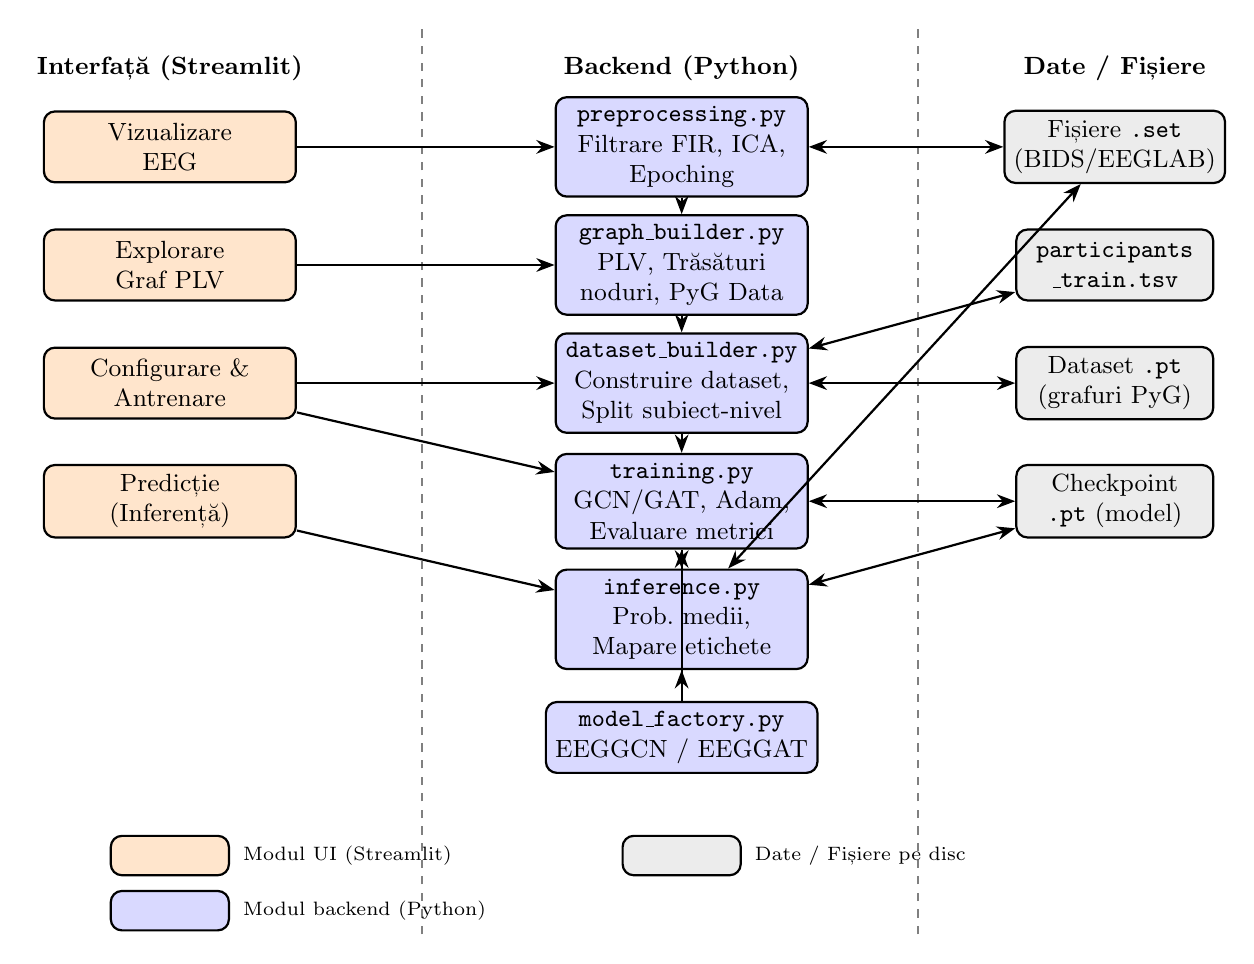
\begin{tikzpicture}[
    box/.style={rectangle, draw=black, rounded corners=4pt,
                minimum width=3.2cm, minimum height=0.9cm,
                align=center, font=\small},
    backend/.style={box, fill=blue!15},
    frontend/.style={box, fill=orange!20},
    data/.style={box, fill=gray!15, minimum width=2.5cm},
    >=Stealth,
    thick
]

%% --- Titluri sectiuni ---
\node[font=\bfseries\small] at (0, 6.5) {Interfață (Streamlit)};
\node[font=\bfseries\small] at (6.5, 6.5) {Backend (Python)};
\node[font=\bfseries\small] at (12.0, 6.5) {Date / Fișiere};

%% --- Linii de separare ---
\draw[dashed, gray] (3.2, -4.5) -- (3.2, 7.0);
\draw[dashed, gray] (9.5, -4.5) -- (9.5, 7.0);

%% --- MODULE INTERFATA ---
\node[frontend] (ui_viz)   at (0, 5.5) {Vizualizare\\EEG};
\node[frontend] (ui_graph) at (0, 4.0) {Explorare\\Graf PLV};
\node[frontend] (ui_train) at (0, 2.5) {Configurare \&\\Antrenare};
\node[frontend] (ui_pred)  at (0, 1.0) {Predicție\\(Inferență)};

%% --- MODULE BACKEND ---
\node[backend] (prep)    at (6.5, 5.5) {\texttt{preprocessing.py}\\Filtrare FIR, ICA,\\Epoching};
\node[backend] (graph)   at (6.5, 4.0) {\texttt{graph\_builder.py}\\PLV, Trăsături\\noduri, PyG Data};
\node[backend] (dataset) at (6.5, 2.5) {\texttt{dataset\_builder.py}\\Construire dataset,\\Split subiect-nivel};
\node[backend] (train)   at (6.5, 1.0) {\texttt{training.py}\\GCN/GAT, Adam,\\Evaluare metrici};
\node[backend] (infer)   at (6.5,-0.5) {\texttt{inference.py}\\Prob.\ medii,\\Mapare etichete};
\node[backend] (factory) at (6.5,-2.0) {\texttt{model\_factory.py}\\EEGGCN / EEGGAT};

%% --- DATE / FISIERE ---
\node[data] (eeg_files) at (12.0, 5.5) {Fișiere \texttt{.set}\\(BIDS/EEGLAB)};
\node[data] (tsv)       at (12.0, 4.0) {\texttt{participants}\\{\texttt{\_train.tsv}}};
\node[data] (pt_data)   at (12.0, 2.5) {Dataset \texttt{.pt}\\(grafuri PyG)};
\node[data] (ckpt)      at (12.0, 1.0) {Checkpoint\\{\texttt{.pt}} (model)};

%% --- SAGETI UI -> BACKEND ---
\draw[->] (ui_viz)   -- (prep);
\draw[->] (ui_graph) -- (graph);
\draw[->] (ui_train) -- (dataset);
\draw[->] (ui_train) -- (train);
\draw[->] (ui_pred)  -- (infer);

%% --- SAGETI BACKEND -> BACKEND ---
\draw[->] (prep)    -- (graph);
\draw[->] (graph)   -- (dataset);
\draw[->] (dataset) -- (train);
\draw[->] (train)   -- (infer);
\draw[->] (factory) -- (train);
\draw[->] (factory) -- (infer);

%% --- SAGETI BACKEND <-> DATE ---
\draw[<->] (prep)    -- (eeg_files);
\draw[<->] (dataset) -- (tsv);
\draw[<->] (dataset) -- (pt_data);
\draw[<->] (train)   -- (ckpt);
\draw[<->] (infer)   -- (ckpt);
\draw[<->] (infer)   -- (eeg_files);

%% --- Legenda ---
\node[frontend, minimum width=1.5cm, minimum height=0.5cm] at (0, -3.5) {};
\node[right, font=\scriptsize] at (0.8, -3.5) {Modul UI (Streamlit)};
\node[backend, minimum width=1.5cm, minimum height=0.5cm] at (0, -4.2) {};
\node[right, font=\scriptsize] at (0.8, -4.2) {Modul backend (Python)};
\node[data, minimum width=1.5cm, minimum height=0.5cm] at (6.5, -3.5) {};
\node[right, font=\scriptsize] at (7.3, -3.5) {Date / Fișiere pe disc};

\end{tikzpicture}
\caption{Diagrama de arhitectură a aplicației grafice interactive dezvoltate cu Streamlit, evidențiind modulele principale și fluxul de date între ele.}
\label{fig:app_diagram}
\end{figure}

\section{Prezentare generală}

Pentru a facilita utilizarea practică a sistemului propus, a fost dezvoltată o interfață grafică interactivă bazată pe framework-ul Streamlit. Alegerea acestei tehnologii este motivată de simplitatea integrării cu ecosistemul Python, de suportul nativ pentru elemente interactive și de capacitatea de a construi rapid aplicații destinate explorării datelor și modelelor de învățare automată.

Interfața are rolul de a conecta utilizatorul cu toate etapele importante ale pipeline-ului implementat: încărcarea și inspectarea semnalelor EEG, vizualizarea conectivității funcționale, configurarea și antrenarea modelelor GNN și realizarea de predicții pe înregistrări noi. Astfel, aplicația nu reprezintă doar o componentă auxiliară, ci un strat de interacțiune care face posibilă utilizarea sistemului într-un mod intuitiv și reproductibil.

Din punct de vedere al organizării interne, aplicația este structurată în două module principale:
\begin{itemize}
    \item fișierul \texttt{app/main.py}, care definește logica principală a aplicației, navigarea între secțiuni și integrarea funcțiilor de procesare, antrenare și inferență;
    \item fișierul \texttt{app/ui\_components.py}, care conține componente reutilizabile pentru interfață, elemente grafice și funcții auxiliare pentru afișarea rezultatelor.
\end{itemize}

Aplicația comunică direct cu modulele backend dezvoltate în capitolele anterioare:
\begin{itemize}
    \item \texttt{src/preprocessing.py} -- pentru încărcarea și pre-procesarea semnalelor EEG;
    \item \texttt{src/graph\_builder.py} -- pentru construirea și vizualizarea grafurilor de conectivitate funcțională;
    \item \texttt{src/dataset\_builder.py} -- pentru generarea setului de date;
    \item \texttt{src/training.py} -- pentru antrenarea și evaluarea modelelor;
    \item \texttt{src/inference.py} -- pentru realizarea predicțiilor.
\end{itemize}

Din perspectiva utilizatorului, interfața este organizată în patru zone funcționale principale:
\begin{enumerate}
    \item vizualizarea semnalelor EEG;
    \item explorarea conectivității funcționale și a grafurilor asociate;
    \item configurarea și antrenarea modelelor;
    \item realizarea predicțiilor pe date noi.
\end{enumerate}

Această împărțire reflectă etapele naturale ale fluxului de lucru și permite utilizatorului să treacă gradual de la inspecția datelor brute la interpretarea rezultatului final al clasificării.

\begin{figure}[H]
    \centering
    \includegraphics[width=0.8\textwidth]{images/App_Homepage.png}
    \caption{Pagina principală a aplicației grafice dezvoltate cu Streamlit.}
    \label{fig:streamlit_main_page}
\end{figure}

\section{Vizualizarea semnalelor EEG}

Una dintre funcționalitățile esențiale ale interfeței este posibilitatea de a inspecta vizual semnalele EEG încărcate. Această componentă este utilă atât pentru verificarea corectitudinii datelor introduse, cât și pentru o înțelegere mai bună a caracteristicilor semnalului înainte de aplicarea etapelor de procesare și clasificare.

Utilizatorul poate selecta un fișier EEG în format \texttt{.set}, iar aplicația îl încarcă folosind aceleași funcții descrise în Secțiunea~3.2. După încărcare, sunt afișate informații descriptive de bază, precum:
\begin{itemize}
    \item numărul de canale disponibile;
    \item lista canalelor selectate;
    \item rata de eșantionare;
    \item durata totală a înregistrării.
\end{itemize}

Pe lângă aceste informații, interfața permite reprezentarea grafică a semnalelor EEG pe canale, pe o durată de timp selectabilă de către utilizator. Această vizualizare este importantă pentru identificarea unor caracteristici evidente ale semnalului, precum fluctuațiile de amplitudine, prezența zgomotului sau eventuale artefacte reziduale.

În plus, aplicația oferă utilizatorului posibilitatea de a vizualiza matricea de conectivitate funcțională calculată prin PLV. Aceasta este afișată sub forma unei hărți de căldură (\textit{heatmap}), în care intensitatea culorii reflectă nivelul de sincronizare dintre perechile de electrozi. O astfel de reprezentare permite observarea rapidă a relațiilor funcționale dominante dintre regiunile cerebrale.

Pornind de la această matrice, aplicația poate genera și o reprezentare explicită a grafului EEG, în care:
\begin{itemize}
    \item nodurile corespund electrozilor;
    \item muchiile reprezintă conexiunile funcționale care depășesc pragul selectat;
    \item grosimea muchiilor este proporțională cu intensitatea PLV.
\end{itemize}

Această componentă are un rol important în interpretarea reprezentării pe graf utilizate de modelele GNN, oferind o legătură directă între semnalul inițial și structura topologică folosită în clasificare.

\begin{figure}[H]
    \centering
    \includegraphics[width=0.8\textwidth]{images/EEG_Channels.png}
    \caption{Modulul de vizualizare a semnalelor EEG în interfața grafică.}
    \label{fig:eeg_signal_view}
\end{figure}

\begin{figure}[H]
    \centering
    \includegraphics[width=0.8\textwidth]{images/Brain_Graph.png}
    \caption{Vizualizarea conectivității funcționale și a grafului EEG asociat unei înregistrări.}
    \label{fig:plv_graph_view}
\end{figure}

\section{Configurarea și antrenarea modelelor}

Interfața include un modul dedicat configurării experimentelor și lansării procesului de antrenare. Scopul acestuia este de a permite utilizatorului să controleze parametrii principali ai modelului și ai pipeline-ului, fără a fi necesară modificarea directă a codului sursă.

Din interfață pot fi configurați, printre alții, următorii parametri:
\begin{itemize}
    \item arhitectura modelului (\texttt{GCN} sau \texttt{GAT});
    \item modul de clasificare (\textit{binary} sau \textit{three\_class});
    \item numărul de epoci de antrenare;
    \item rata de învățare;
    \item dimensiunea batch-ului;
    \item dimensiunea spațiului latent;
    \item probabilitatea de \textit{dropout};
    \item pragul PLV utilizat la construirea grafurilor;
    \item durata ferestrei temporale folosite în segmentare.
\end{itemize}

În cazul modelului GAT, utilizatorul poate specifica suplimentar numărul de capuri de atenție utilizate în fiecare strat. Această flexibilitate permite explorarea mai multor configurații experimentale și compararea comportamentului celor două arhitecturi implementate.

După configurare, utilizatorul poate lansa procesul de antrenare direct din interfață. În timpul execuției, aplicația afișează în timp real informații despre progresul antrenării, precum:
\begin{itemize}
    \item epoca de antrenare curentă;
    \item pierderea medie pe antrenare;
    \item acuratețea pe validare;
    \item valorile macro pentru precizie, recall și scor F1;
    \item cea mai bună performanță obținută până în acel moment.
\end{itemize}

Această monitorizare în timp real este utilă pentru identificarea comportamentului modelului pe parcursul antrenării și pentru detectarea unor posibile probleme, precum stagnarea performanței sau supraînvățarea.

La finalul procesului, aplicația afișează un rezumat al experimentului, incluzând cea mai bună epocă de antrenare și valorile finale ale metricilor. În plus, checkpoint-urile salvate pot fi utilizate ulterior atât pentru analiză, cât și pentru inferență.

\begin{figure}[H]
    \centering
    \includegraphics[width=0.8\textwidth]{images/Training_Config.png}
    \caption{Panoul de configurare a hiperparametrilor și de lansare a antrenării.}
    \label{fig:training_config_panel}
\end{figure}

\begin{figure}[H]
    \centering
    \includegraphics[width=0.8\textwidth]{images/Training_Progress.png}
    \caption{Afișarea progresului antrenării și a metricilor calculate pe parcursul procesului de optimizare.}
    \label{fig:training_progress}
\end{figure}

\section{Realizarea predicțiilor}

Un alt modul important al aplicației este cel dedicat inferenței pe înregistrări EEG noi. Acesta permite utilizatorului să încarce un fișier necunoscut modelului și să obțină o predicție automată privind clasa clinică asociată.

Fluxul de lucru urmat în această secțiune reproduce pașii descriși în Secțiunea~3.7:
\begin{enumerate}
    \item selectarea unui checkpoint antrenat anterior;
    \item încărcarea unei înregistrări EEG noi;
    \item aplicarea pre-procesării standard;
    \item segmentarea în ferestre temporale;
    \item construirea grafurilor corespunzătoare;
    \item clasificarea fiecărei ferestre temporale;
    \item agregarea predicțiilor prin probabilități medii.
\end{enumerate}

Rezultatul final este afișat sub forma unei etichete clinice ușor de interpretat, împreună cu distribuția predicțiilor pe ferestre temporale. De exemplu, utilizatorul poate vedea nu doar clasa prezisă final, ci și câte segmente temporale au fost clasificate în fiecare categorie.

Această prezentare oferă un nivel suplimentar de transparență și permite identificarea situațiilor în care predicția este stabilă sau, dimpotrivă, ambiguă. În plus, interfața poate afișa și probabilitățile asociate claselor, oferind o imagine mai nuanțată asupra încrederii modelului în rezultatul furnizat.

Prin această componentă, aplicația depășește rolul unui simplu instrument experimental și se apropie de un prototip funcțional destinat analizei asistate a semnalelor EEG. Integrarea inferenței în interfața grafică contribuie semnificativ la accesibilitatea sistemului și la potențialul său de utilizare în contexte educaționale sau de cercetare aplicată.

\begin{figure}[H]
    \centering
    \includegraphics[width=0.8\textwidth]{images/Diagnosis_Settings.png}
    \caption{Panoul de configurare pentru realizarea predicțiilor.}
    \label{fig:configuration_panel}
\end{figure}

\begin{figure}[H]
    \centering
    \includegraphics[width=0.8\textwidth]{images/Diagnosis_Result.png}
    \caption{Panoul de afișare a rezultatelor pentru realizarea predicțiilor.}
    \label{fig:results_panel}
\end{figure}

\begin{figure}[H]
    \centering
    \includegraphics[width=0.8\textwidth]{images/Diagnosis_Visualization.png}
    \caption{Panoul de vizualizare a rezultatelor pentru realizarea predicțiilor.}
    \label{fig:visualization_panel}
\end{figure}

\begin{figure}[H]
    \centering
    \includegraphics[width=0.8\textwidth]{images/Per_Window_Predictions.png}
    \caption{Tabelul de afișare a rezultatelor pentru realizarea predicțiilor per fereastră temporală.}
    \label{fig:per_window_predictions}
\end{figure}

\section{Observații privind utilitatea interfeței}

Interfața grafică dezvoltată în cadrul acestei lucrări are un rol important nu doar din perspectiva utilizării practice, ci și din perspectiva validării și interpretării întregului sistem propus. Prin centralizarea etapelor de încărcare, pre-procesare, construire a grafurilor, antrenare și inferență într-un singur mediu interactiv, aplicația facilitează explorarea comportamentului modelelor și verificarea coerenței rezultatelor obținute.

De asemenea, această interfață contribuie la creșterea accesibilității soluției dezvoltate. Utilizatorii care nu sunt familiarizați cu detaliile implementării la nivel de cod pot interacționa cu sistemul într-un mod intuitiv, configurând experimente și analizând rezultate prin elemente vizuale și controale simple. În același timp, integrarea directă cu modulele backend garantează faptul că interfața utilizează exact aceleași proceduri de procesare și clasificare descrise în capitolele anterioare.

În concluzie, interfața grafică reprezintă o extensie firească a pipeline-ului propus, transformând o implementare experimentală într-un sistem mai ușor de utilizat, de analizat și de demonstrat în contexte academice sau aplicative.

% ============================================================
% CAPITOLUL 5 — REZULTATE EXPERIMENTALE
% ============================================================
\chapter{Rezultate experimentale}

Prezentul capitol prezintă evaluarea cantitativă a modelelor implementate. Sunt raportate
metricile de validare la nivel de fereastră temporală, rezultatele inferenței pe subiecți
din setul holdout și o analiză comparativă care evidențiază impactul tipului de
conectivitate și al arhitecturii asupra performanței.

\section{Configurația experimentală}
\label{sec:config_exp}

Experimentele au fost realizate pe setul de date descris în Secțiunea~3.1, utilizând
înregistrări EEG resting-state (protocol \textit{eyes-closed}), 19 canale din sistemul
10-20, stocate în format BIDS. Împărțirea datelor s-a realizat la nivel de subiect
(80\% antrenare / 20\% validare), eliminând riscul de \textit{data leakage}.

Au fost evaluate patru combinații de model și tip de conectivitate, pe două scenarii
de clasificare:

\begin{itemize}
    \item \textbf{Conectivitate funcțională (PLV)} vs. \textbf{Conectivitate topologică
          (proximitate spațială 10-20)};
    \item \textbf{GCN} vs. \textbf{GAT};
    \item \textbf{Clasificare binară} (Healthy Control vs. Alzheimer's Disease) vs.
          \textbf{Clasificare pe trei clase} (HC vs. AD vs. FTD).
\end{itemize}

Dimensiunile seturilor de date construite sunt sintetizate în Tabelul~\ref{tab:dataset_size}.

\begin{table}[H]
    \centering
    \caption{Dimensiunea seturilor de date utilizate în experimente.}
    \label{tab:dataset_size}
    \begin{tabular}{|l|c|c|c|}
        \hline
        \textbf{Mod} & \textbf{Nr. grafuri total} & \textbf{Subiecți antrenare} & \textbf{Subiecți validare} \\
        \hline
        Binar (C vs.\ A) & 22\,888 & 50 & 13 \\
        \hline
        3 clase (C/A/F) & 30\,022 & 68 & 17 \\
        \hline
    \end{tabular}
\end{table}

Hiperparametrii comuni tuturor experimentelor sunt: dimensiune latentă $H = 64$,
dropout $= 0.5$, optimizator Adam cu weight decay $10^{-4}$, scheduler
\texttt{ReduceLROnPlateau} (patience $= 10$, factor $= 0.5$), funcție de pierdere
\texttt{CrossEntropyLoss} cu ponderi inverse frecvenței de clasă.

% ============================================================
\section{Rezultate la nivel de fereastră temporală}
\label{sec:rezultate_fereastra}

Metricile raportate sunt macro-averaged (medie egală pe clase), calculate pe setul de
validare al fiecărui model. Valoarea reținută corespunde epocii cu acuratețea maximă pe
validare (\textit{best checkpoint}).

\subsection{Clasificare binară (Healthy Control vs.\ Alzheimer's Disease)}

\begin{table}[H]
    \centering
    \caption{Rezultate de validare pentru clasificarea binară (C vs.\ A).}
    \label{tab:rezultate_binar}
    \begin{tabular}{|l|c|c|c|c|c|c|}
        \hline
        \textbf{Conectivitate} & \textbf{Model} & \textbf{Accuracy} & \textbf{Precision} & \textbf{Recall} & \textbf{F1} & \textbf{Epocă} \\
        \hline
        Funcțională & GCN   & 71,0\% & 0,751 & 0,746 & 0,710 & 7  \\
        Funcțională & \textbf{GAT} & \textbf{73,8\%} & \textbf{0,741} & \textbf{0,751} & \textbf{0,736} & 25 \\
        Topologică  & GCN   & 66,9\% & 0,721 & 0,709 & 0,668 & 7  \\
        Topologică  & GAT   & 71,1\% & 0,728 & 0,734 & 0,710 & 38 \\
        \hline
    \end{tabular}
\end{table}

Cel mai bun model în scenariul binar este \textbf{GAT cu conectivitate funcțională},
cu o acuratețe de 73,8\% și F1 macro de 0,736. Se observă că GAT depășește GCN în
ambele tipuri de conectivitate, iar conectivitatea funcțională (PLV) conduce la
performanțe superioare față de cea topologică pentru ambele arhitecturi.

\subsection{Clasificare pe trei clase (HC vs.\ AD vs.\ FTD)}

\begin{table}[H]
    \centering
    \caption{Rezultate de validare pentru clasificarea pe trei clase (C/A/F).}
    \label{tab:rezultate_3clase}
    \begin{tabular}{|l|c|c|c|c|c|c|}
        \hline
        \textbf{Conectivitate} & \textbf{Model} & \textbf{Accuracy} & \textbf{Precision} & \textbf{Recall} & \textbf{F1} & \textbf{Epocă} \\
        \hline
        Funcțională & GCN   & 56,0\% & 0,579 & 0,627 & 0,510 & 5  \\
        Funcțională & \textbf{GAT} & \textbf{60,8\%} & \textbf{0,611} & \textbf{0,639} & \textbf{0,564} & 22 \\
        Topologică  & GCN   & 52,1\% & 0,435 & 0,556 & 0,418 & 1  \\
        Topologică  & GAT   & 60,5\% & 0,546 & 0,630 & 0,555 & 49 \\
        \hline
    \end{tabular}
\end{table}

Scenariul cu trei clase este semnificativ mai dificil, acuratețea maximă atingând
60,8\% (GAT funcțional). Scorul F1 macro scăzut al modelului GCN topologic (0,418)
indică o convergență rapidă spre o soluție suboptimală, confirmată de faptul că
\textit{best checkpoint} a fost salvat la prima epocă.

% ============================================================
\section{Rezultate la nivel de subiect (inferență pe holdout)}
\label{sec:rezultate_holdout}

Pentru evaluarea capacității de generalizare la nivel clinic, au fost testate trei
subiecți din setul holdout, cu diagnostice reale cunoscute: \textbf{sub-024}
(Alzheimer's Disease), \textbf{sub-055} (Healthy Control) și \textbf{sub-070}
(Frontotemporal Dementia). Predicția finală pentru fiecare subiect a fost obținută
prin agregarea probabilităților medii pe toate ferestrele temporale ale înregistrării,
conform Ecuației~\eqref{eq:prob_aggregation}.

\begin{table}[H]
    \centering
    \caption{Rezultatele inferenței pe setul holdout. C = Healthy Control,
             A = Alzheimer's Disease, F = Frontotemporal Dementia.}
    \label{tab:holdout}
    \begin{tabular}{|l|l|c|c|c|c|c|}
        \hline
        \textbf{Subiect} & \textbf{Diagnostic real} & \textbf{Conectivitate} & \textbf{Model} & \textbf{Mod} & \textbf{Predicție} & \textbf{Confidență} \\
        \hline
        sub-024 & AD & Funcțională & GCN & Binar   & AD & 86,2\% \\
        sub-024 & AD & Funcțională & GAT & Binar   & AD & 88,4\% \\
        sub-024 & AD & Topologică  & GCN & Binar   & AD & 74,8\% \\
        sub-024 & AD & Topologică  & GAT & Binar   & AD & 87,3\% \\
        sub-024 & AD & Funcțională & GCN & 3 clase & AD & 55,8\% \\
        sub-024 & AD & Funcțională & GAT & 3 clase & AD & 57,1\% \\
        sub-024 & AD & Topologică  & GCN & 3 clase & AD & 51,3\% \\
        sub-024 & AD & Topologică  & GAT & 3 clase & AD & 64,9\% \\
        \hline
        sub-055 & HC & Funcțională & GCN & Binar   & HC & 80,0\% \\
        sub-055 & HC & Funcțională & GAT & Binar   & HC & 69,5\% \\
        sub-055 & HC & Topologică  & GCN & Binar   & HC & 77,9\% \\
        sub-055 & HC & Topologică  & GAT & Binar   & HC & 82,2\% \\
        sub-055 & HC & Funcțională & GCN & 3 clase & HC & 60,5\% \\
        sub-055 & HC & Funcțională & GAT & 3 clase & HC & 53,1\% \\
        sub-055 & HC & Topologică  & GCN & 3 clase & HC & 48,4\% \\
        sub-055 & HC & Topologică  & GAT & 3 clase & HC & 48,3\% \\
        \hline
        sub-070 & FTD & Funcțională & GCN & 3 clase & HC & 34,5\% \\
        sub-070 & FTD & Funcțională & GAT & 3 clase & AD & 35,0\% \\
        sub-070 & FTD & Topologică  & GCN & 3 clase & AD & 37,6\% \\
        sub-070 & FTD & Topologică  & GAT & 3 clase & AD & 41,1\% \\
        \hline
    \end{tabular}
\end{table}

Sumarul acurateței la nivel de subiect este prezentat în Tabelul~\ref{tab:holdout_summary}.

\begin{table}[H]
    \centering
    \caption{Sumarul acurateței la nivel de subiect pe setul holdout.}
    \label{tab:holdout_summary}
    \begin{tabular}{|l|c|c|c|}
        \hline
        \textbf{Categorie} & \textbf{Corecte} & \textbf{Total} & \textbf{Acuratețe} \\
        \hline
        Modele binare (sub-024, sub-055) & 8 & 8 & \textbf{100\%} \\
        \hline
        Modele 3-clase (sub-024, sub-055, sub-070) & 8 & 12 & \textbf{66,7\%} \\
        \hline
        \textbf{Total} & \textbf{16} & \textbf{20} & \textbf{80\%} \\
        \hline
    \end{tabular}
\end{table}

Toate cele opt rulări în modul binar au clasificat corect ambii subiecți testați,
cu confidențe cuprinse între 69,5\% și 88,4\%, ceea ce indică o separare robustă
între clasa Alzheimer și cea sănătoasă. În modul cu trei clase, subiecții sub-024
(AD) și sub-055 (HC) au fost clasificați corect de toate modelele, în timp ce
sub-070 (FTD) nu a fost clasificat corect de niciun model, cu confidențe la nivel
de șansă (34--41\%), indicând ambiguitate ridicată în predicție.

% ============================================================
\section{Analiză comparativă și discuții}
\label{sec:discutii}

\textbf{Conectivitate funcțională vs.\ topologică.} În toate configurațiile testate,
conectivitatea funcțională bazată pe PLV a condus la performanțe egale sau superioare
față de conectivitatea topologică. Diferența este mai pronunțată în cazul GCN (71,0\%
vs.\ 66,9\% la binar; 56,0\% vs.\ 52,1\% la 3 clase), sugerând că sincronizarea
de fază în banda Alpha captează tipare discriminative pe care simpla proximitate
anatomică a electrozilor nu le poate oferi.

\textbf{GAT vs.\ GCN.} Modelul GAT depășește GCN în toate cele patru combinații
de conectivitate și mod de clasificare. Avantajul este mai consistent în regimul cu
trei clase, unde mecanismul de atenție adaptivă permite modelului să se concentreze
pe conexiunile relevante între regiuni cerebrale, reducând impactul zgomotului structural.

\textbf{Binar vs.\ trei clase.} Trecerea de la clasificarea binară la cea cu trei clase
produce o scădere semnificativă a acurateței (de la $\sim$73\% la $\sim$61\% pentru cel
mai bun model). Scăderea este explicată parțial de dimensiunea mai mică a clasei FTD
în setul de antrenare și de suprapunerea parțială a semnăturii EEG a FTD cu cea a AD,
ambele afecțiuni prezentând modificări similare în banda Theta și Delta.

\textbf{Cazul sub-070 (FTD).} Eșecul tuturor modelelor în clasificarea subiectului
FTD, cu confidențe scăzute (34--41\%), nu este neapărat surprinzător în contextul
setului de date disponibil. Clasa FTD este sub-reprezentată numeric față de AD și HC,
iar trăsăturile spectrale utilizate (puterea pe patru benzi) pot fi insuficiente pentru
a distinge FTD de AD la nivel individual. Aceste observații indică direcții clare de
îmbunătățire, discutate în Capitolul~6.

\textbf{Limite ale evaluării.} Setul holdout conține doar trei subiecți, ceea ce face
ca rezultatele la nivel de subiect să fie ilustrative, nu statistic concludente.
Baza cantitativă solidă a evaluării rămâne metricile macro-averaged pe setul de
validare (Tabelele~\ref{tab:rezultate_binar} și~\ref{tab:rezultate_3clase}), calculate
pe 13, respectiv 17 subiecți nevăzuți în antrenare.

% ============================================================
% CAPITOLUL 6 — CONCLUZII ȘI DIRECȚII VIITOARE
% ============================================================
\chapter{Concluzii și direcții viitoare de dezvoltare}

Prezentul capitol sintetizează contribuțiile principale ale lucrării, discută
limitările identificate pe parcursul procesului de implementare și evaluare și
propune direcții de cercetare și dezvoltare viitoare.

% ============================================================
\section{Concluzii}

Această lucrare a investigat utilizarea rețelelor neuronale de tip graf pentru
analiza și clasificarea semnalelor EEG asociate afecțiunilor neurodegenerative,
cu accent pe boala Alzheimer și demența frontotemporală. Pornind de la natura
non-euclidiană a datelor EEG, a fost propus și implementat un pipeline complet
care transformă înregistrările brute în grafuri procesabile de modele GNN, prin
extragerea puterii spectrale pe benzi de frecvență ca trăsături nodale și
utilizarea Phase Locking Value în banda Alpha ca măsură de conectivitate funcțională
pentru definirea muchiilor.

Au fost implementate și evaluate comparativ două arhitecturi: \textbf{EEGGCN}
(Graph Convolutional Network cu trei straturi, conexiuni reziduale și dual pooling)
și \textbf{EEGGAT} (Graph Attention Network cu mecanism multi-head și conexiune
reziduală cu proiecție liniară). Evaluarea a acoperit patru axe de comparație:
tipul de conectivitate (funcțională vs.\ topologică), arhitectura modelului
(GCN vs.\ GAT), modul de clasificare (binar vs.\ trei clase) și generalizarea
la subiecți nevăzuți (setul holdout).

Principalele concluzii susținute de rezultatele experimentale sunt:

\begin{enumerate}
    \item \textbf{Conectivitatea funcțională (PLV) este superioară celei topologice.}
    În toate configurațiile testate, grafurile construite pe baza sincronizării de
    fază în banda Alpha au condus la performanțe mai bune față de grafurile bazate
    pe proximitatea anatomică a electrozilor. Aceasta confirmă că modificările de
    conectivitate funcțională inter-regională constituie un semnal discriminativ
    relevant pentru detecția afecțiunilor neurodegenerative.

    \item \textbf{GAT depășește GCN în mod consistent.} Mecanismul de atenție
    adaptivă permite modelului GAT să diferențieze importanța conexiunilor în
    funcție de context, ceea ce se traduce într-un avantaj de 2--5 puncte
    procentuale față de GCN, mai pronunțat în scenariul cu trei clase.

    \item \textbf{Clasificarea binară HC vs.\ AD este robustă.} Cel mai bun model
    (GAT funcțional) atinge o acuratețe de 73,8\% și F1 macro de 0,736 la nivel
    de fereastră temporală, cu o acuratețe de 100\% la nivel de subiect pe setul
    holdout, cu confidențe de 69--88\%. Aceste rezultate demonstrează că
    semnalele EEG resting-state, prelucrate prin pipeline-ul propus, conțin
    informație suficientă pentru a distinge subiecții sănătoși de cei cu boala
    Alzheimer.

    \item \textbf{Clasificarea cu trei clase rămâne o provocare.} Acuratețea
    maximă de 60,8\% și eșecul tuturor modelelor în clasificarea subiectului FTD
    (cu confidențe de 34--41\%) indică limitele abordării actuale în fața
    dezechilibrului de clase și a suprapunerii semnăturilor spectrale dintre AD
    și FTD.

    \item \textbf{Interfața grafică interactivă} dezvoltată cu Streamlit
    transformă sistemul dintr-un experiment de cercetare într-un prototip
    funcțional, accesibil utilizatorilor fără expertiză în programare, și
    demonstrează potențialul aplicativ al soluției propuse.
\end{enumerate}

În ansamblu, lucrarea demonstrează că rețelele neuronale de tip graf, combinate
cu o reprezentare adecvată a datelor EEG bazată pe conectivitate funcțională,
reprezintă o alternativă promițătoare față de metodele tradiționale de clasificare
a semnalelor neurofiziologice.

% ============================================================
\section{Limitări identificate}

Pe parcursul implementării și evaluării au fost identificate mai multe limitări
care trebuie luate în considerare la interpretarea rezultatelor:

\begin{itemize}
    \item \textbf{Dimensiunea setului de date.} Setul utilizat conține 85 de
    subiecți în total (63 pentru antrenare în modul binar), o dimensiune relativ
    mică pentru antrenarea modelelor de învățare profundă. Numărul redus de
    subiecți FTD contribuie direct la dificultatea clasificării acestei clase.

    \item \textbf{Setul holdout mic.} Evaluarea la nivel de subiect s-a realizat
    pe trei subiecți, ceea ce nu permite formularea unor concluzii statistice
    generale. Rezultatele holdout sunt ilustrative și complementare metricilor
    de validare.

    \item \textbf{Trăsături nodale limitate.} Vectorul de trăsături al fiecărui
    nod conține doar puterea spectrală pe patru benzi. Informații suplimentare,
    precum coerența, entropia sau trăsăturile de fază, ar putea îmbunătăți
    capacitatea discriminativă a modelului.

    \item \textbf{Conectivitate PLV pe o singură bandă.} Calculul PLV s-a
    realizat exclusiv în banda Alpha. Extinderea la multiple benzi ar produce
    reprezentări de graf mai bogate, la costul unei complexități computaționale
    mai ridicate.

    \item \textbf{Absența ICA în pipeline-ul implicit.} Curățarea artefactelor
    prin ICA este dezactivată implicit din cauza riscului de eliminare accidentală
    a componentelor cerebrale relevante în absența validării manuale. Un protocol
    automat de detecție a artefactelor ar îmbunătăți calitatea datelor de intrare.

    \item \textbf{Lipsa unui set de test independent.} Evaluarea a utilizat
    același set de validare atât pentru selecția hiperparametrilor, cât și pentru
    raportarea metricilor finale, ceea ce poate introduce o supraestimare
    moderată a performanței raportate.
\end{itemize}

% ============================================================
\section{Direcții viitoare de dezvoltare}

Pe baza concluziilor și limitărilor identificate, sunt propuse următoarele
direcții de extindere a lucrării:

\begin{enumerate}
    \item \textbf{Extinderea setului de date și augmentarea.} Includerea unor
    seturi de date publice suplimentare (de exemplu, TUEG, CAUEEG) și aplicarea
    unor tehnici de augmentare mai avansate (mixup la nivel de graf, perturbări
    ale structurii grafului) ar putea crește robustedea și capacitatea de
    generalizare a modelelor.

    \item \textbf{Conectivitate multi-bandă.} Construirea unor grafuri multi-layer
    în care fiecare strat corespunde unei benzi de frecvență ar permite capturarea
    simultană a dinamicii spectrale la diferite scale temporale, o abordare recent
    investigată în literatura de specialitate \cite{klepl2023gnn}.

    \item \textbf{Trăsături nodale îmbogățite.} Adăugarea unor trăsături
    suplimentare la nivelul nodurilor — precum entropia spectrală, indicii de
    complexitate (Higuchi, Hjorth) sau trăsături de conectivitate locală — ar
    putea crește puterea discriminativă a reprezentărilor de graf.

    \item \textbf{Modele spațio-temporale.} Integrarea unei componente temporale
    explicite, prin arhitecturi de tip ST-GNN (Spatio-Temporal GNN) sau prin
    combinarea GNN cu rețele recurente (LSTM, GRU), ar permite exploatarea
    dinamicii temporale a semnalelor EEG, dincolo de caracterizarea spectrală
    per fereastră \cite{rahman2025advancement}.

    \item \textbf{Tehnici de echilibrare a claselor.} Pentru a aborda
    dezechilibrul clasei FTD, pot fi utilizate tehnici de supraesantionare la
    nivel de graf (SMOTE-GNN), generare de date sintetice sau ajustarea dinamică
    a ponderilor de clasă în timpul antrenării.

    \item \textbf{Interpretabilitate.} Integrarea unor metode de explicabilitate
    specifice grafurilor, precum GNNExplainer sau Grad-CAM adaptat pentru GNN,
    ar permite identificarea electrozilor și conexiunilor cu cea mai mare
    contribuție la decizia modelului, crescând relevanța clinică a sistemului
    \cite{hu2024self}.

    \item \textbf{Validare clinică.} O evaluare pe un set de date mai mare,
    cu protocol de validare încrucișată la nivel de subiect și implicarea unor
    experți clinici în analiza rezultatelor, reprezintă pasul necesar pentru
    a transforma prototipul actual într-un instrument cu potențial de utilizare
    în practica medicală.
\end{enumerate}

\bibliography{mybib}
\bibliographystyle{ieeetr}
%\bibliographystyle{alpha}
\addcontentsline{toc}{chapter}{Bibliografie}

\end{document}